\documentclass[11pt,letter]{article}

\usepackage[margin=1in]{geometry}
\usepackage{graphicx}
\usepackage{amssymb}
\usepackage{amsmath}
\usepackage{epstopdf}
\usepackage{setspace}
\usepackage{currfile}
\usepackage[abbr]{harvard}
\usepackage[pagewise]{lineno}
\usepackage{algorithm}
\usepackage{algorithmic}
\usepackage{array,booktabs}

\DeclareMathOperator{\var}{Var}
\DeclareMathOperator{\cov}{Cov}
\DeclareMathOperator{\diag}{diag}

\newcommand{\Dpi}{Dirichlet RP model}
\newcommand{\DP}{Dirichlet RC model}

\newtheorem{theorem}{Theorem}[section]
\newtheorem{lemma}[theorem]{Lemma}
\newtheorem{proposition}[theorem]{Proposition}
\newtheorem{corollary}[theorem]{Corollary}

\newenvironment{proof}[1][Proof]{\begin{trivlist}
\item[\hskip \labelsep {\bfseries #1}]}{\end{trivlist}}
\newenvironment{definition}[1][Definition]{\begin{trivlist}
\item[\hskip \labelsep {\bfseries #1}]}{\end{trivlist}}
\newenvironment{example}[1][Example]{\begin{trivlist}
\item[\hskip \labelsep {\bfseries #1}]}{\end{trivlist}}
\newenvironment{remark}[1][Remark]{\begin{trivlist}
\item[\hskip \labelsep {\bfseries #1}]}{\end{trivlist}}

\usepackage{hyperref}
\hypersetup{
    colorlinks,
    citecolor=black,
    filecolor=black,
    linkcolor=black,
    urlcolor=black
}
\usepackage{authblk}

%\setpagewiselinenumbers
%\modulolinenumbers[5]
%\linenumbers
%\doublespace
%\setstretch{1.5}

\title{Sequential Monte Carlo for random preferences}
\author[1]{William J. McCausland\thanks{william.j.mccausland@umontreal.ca, File: \texttt{\currfilename}.}}
\affil[1]{Universit\'e de Montr\'eal}

\begin{document}

\maketitle

\newtheorem{thm}{Theorem}
\newtheorem{defn}{Definition}

\begin{abstract}
We show how to use Sequential Monte Carlo (SMC) simulation methods to compute marginal likelihoods for an abstract discrete Bayesian random choice model, an abstract Bayesian random preference model, and a collection of hybrid models.
This allows us to compare the models using Bayes factors, which measure relative out-of-sample predictive performance.
For each menu from a given universe of objects, these models all share the same (explicit for the random choice model, implicit for the others) marginal prior distribution of the choice probabilities on that menu.
This allows for a clean comparison of models, based only on how they differ in the degree of dependence of choice probabilities across menus.
Using data from a discrete choice experiment featuring 32 choice domains and 1042 participants, we find strong evidence in favour of the random preference model.
It dominates the random choice model for all choice domains.
For 31 domains it dominates all hybrid models and in the other domain, it is still competitive with the best hybrid model.
%We consider stochastic choice from menus of options taken from a finite universe $T$.
%We introduce computational methods for comparing a Bayesian random preference (RP) model against a Bayesian random choice (RC) model.
%The RP model consists of a class of prior distributions, indexed by a parameter $\alpha \in (0,\infty)$, over the set of random preferences on $T$.
%We show that these distributions, and only these, satisfy a set of symmetry and neutrality properties.
%The RC model consists of a class of priors, also indexed by $\alpha$, over the set (one for each menu) of choice probability vectors.
%For given $\alpha$, and each menu $A$, the implied marginal prior for the choice probability vector on $A$ in the RP model coincides with the explicit marginal prior in the RC model.
%To compare models we compute Bayes factors, through Sequential Monte Carlo (SMC) simulation of a sequence of hybrid distributions bridging the posterior distribution of the RC model and that of the RC model.
%We find strong evidence in favour of the RP model for a data set from a discrete choice experiment featuring 32 choice universes and 1042 participants.
\end{abstract}

\section{Introduction}

Let $T = \{x_1,\dots,x_n\}$ be a finite universe of choice options.
In a choice trial, a decision maker (DM) faces a menu, some non-empty subset of $T$, and must choose a single option from that menu.
The probability that the DM chooses $x \in A$ when presented with menu $A$ is denoted $P_A(x)$.
A {\em random choice} (RC) model on $T$ is the complete specification of the $P_A(x)$, $x \in A \subseteq T$, and is denoted $P$.
A RC model may describe the choices of a single DM over multiple trials, or those of a sample of DMs from a population.
We assume choices are independent across trials.
This is an innocuous assumption for experiments, such as the one we study here, with between-subject designs.

Discrete choice models are used extensively in economics, psychology, marketing, and other disciplines.
Most of these models are random utility models, in which utilities of options are random, and choices maximize realized utility.
Not all random choice models satisfy random utility; that is, not all systems of choice probabilities can be induced by a random utility model.
In fact, random utility is a very restrictive condition and there is some unfavourable empirical evidence, most notably the asymmetric dominance effect, described by \citeasnoun{HubePaynPuto82} and observed in some choice environments.
See \citeasnoun{McCaStobMarlParkBrow20} and the literature cited there for elaboration and support of these claims.

This paper is part of a research agenda devoted to testing random utility and other conditions relating choice probabilities across different menus of options, such as weak stochastic transitivity.
Our investigation of random choice, and the random utility condition in particular, is guided by the following principles.
First, we take choice options to be {\em a priori} indistinguishable, allowing us to focus more on patterns and regularities in choice probabilities that apply universally across choice environments, rather than how attributes of choice options affect choice in particular cases.
To test the random utility condition, we do not rely on parametric random utility models, including models where the random utility distribution depends on observed choice attributes, useful as these models are for applied work.
Such models may be misspecified, and so a poor fit to data does not imply that random utility does not hold.
Second, we do not limit ourselves to tests of particular necessary conditions, such as the condition, necessary for random utility, violated when the asymmetric dominance effect occurs.
Third, we prefer to use data where we observe choices from all non-empty subsets of a universe of objects.
This is because random utility, and other conditions, constrain choice probabilities over all menus.
As they relate to random utility, we can summarize these three principles as follows: we want to test random utility, no more and no less, exposing every implication of random utility to possible falsification.

We test the random utility condition indirectly, by testing the equivalent\footnote{See \citeasnoun{MarlRege18}, noting the requirement, satisfied here, that the universe be countable.} random preference condition, the condition that choice probabilities can be induced by a random preference (RP) model, in which preference are random and a DM chooses the most preferred option from any given menu.
The test is a comparison of two discrete choice models introduced by \citeasnoun{McCaMarl13}, with a common scalar parameter $\alpha \in (0,\infty)$.
The first, which we will call the \Dpi{}, is a Bayesian RP model consisting of a symmetric Dirichlet prior distribution for the vector of $n!$ preference probabilities.
The implicit marginal prior distribution of each $P_A(\cdot)$ is also symmetric Dirichlet and the Dirichlet parameter associated with each option in $A$ is the constant $\alpha/|A|$.
The second, which we will call the \DP{}, is a Bayesian RC model consisting of a prior distribution over the set of choice probability vectors $P_A(\cdot)$, $\emptyset \neq A \subseteq T$.
The (explicit) marginal prior distribution of each $P_A(\cdot)$ is the same symmetric Dirichlet distribution as the implicit marginal prior distribution of $P_A(\cdot)$ in the \Dpi{}, but here the $P_A(\cdot)$ are mutually independent across menus.
Both models are non-parametric, in the sense that the two priors have full support on the set of RP and RC models, respectively.

The present paper makes several contributions.
We show that the symmetric Dirichlet prior distributions of the \Dpi{} and only these distributions, satisfy a set of three desirable properties we call full support, symmetry in preferences and neutrality with respect to all partitions.
We point out that these prior distributions satisfy another, qualitative, property that does not obviously follow from the other three properties, that the marginal distribution of each preference probability resembles a spike-and-slab sparseness prior.
We introduce a new\footnote{The hybrid model here is an improvement on a hybrid model introduced in \citeasnoun{McCaMarl13}.} hybrid model, indexed by $\alpha$ and an additional scalar parameter $\lambda \in [0,1]$, bridging the \DP{} ($\lambda = 0$) and the \Dpi{} ($\lambda = 1$).
We introduce new Sequential Monte Carlo (SMC) methods to simulate the posterior distributions of a sequence of models indexed by values of $\lambda$ increasing from zero to one.
These methods deliver marginal likelihoods for the \DP{}, the \Dpi{} and the hybrid models.
The marginal likelihood for a model measures its out-of-sample predictive performance for a given data set.
Having marginal likelihoods for these models allows direct comparisons using Bayes factors, not only among them, but also with any other model for which one can compute a marginal likelihood.
Finally, we apply our methods to data from a discrete choice experiment featuring 32 choice universes and 1042 participants and report results.
We find the out-of-sample predictive performance of the \Dpi{} to be superior to that of the \DP{}, and we put the degree of superiority in the larger context of how much different features of abstract choice models contribute to predictive success.

\subsection{Random choice, random utility and random preference}

A {\em choice dataset} for a universe $T$ consists of choices observed from various menus, non-empty subsets of $T$, over a number of trials.
We denote the full dataset as $y$, and the choice data observed for each menu $A$ as $y_A$.
Instead of being more specific about the structure of $y$ and the $y_A$, we will introduce notation for a set of count statistics that, in any model where choices are governed by some RC model $P$ and the independence assumption, is a sufficient statistic for $P$.
For all $x \in A \subseteq T$, let $N_A(x)$ be the number of times $x$ is chosen from menu $A$; let $N$ be the complete specification of the $N_A(x)$, a sufficient statistic for $P$.
We can write the conditional probability mass function for data $y$ generated by a RC model $P$ as
\begin{equation}\label{e:likeP}
  f_\mathrm{RC}(y|P) \equiv \prod_{\emptyset \neq A \subseteq T} f_\mathrm{RC}(y_A|P_A) \equiv \prod_{\emptyset \neq A \subseteq T} \prod_{x \in A} P_A(x)^{N_A(x)}.
\end{equation}

A particular RC model may or may not satisfy the random utility and random preference conditions, which are equivalent to each other.
To define them, we first need to define random utility models and random preference models.

\begin{defn}
    A {\em random utility} (RU) model for a universe $T$ is a probability space $(\Omega,{\cal F},\mu)$, where $\Omega$ is a sample space, ${\cal F}$ is an event space and $\mu$ is a probability measure on ${\cal F}$; and a measurable {\em utility} function $u\colon T \times \Omega \rightarrow \mathbb{R}$, where $\mu$ is {\em non-coincident}, meaning that for all distinct $x,y \in T$,
\[
    \mu\left(\{\omega \in \Omega \colon u(x,\omega) = u(y,\omega)\}\right)
    = 0.
\]
\end{defn}

Maximization of $u(\cdot;\omega)$ governs choice in state $\omega$; the non-coincidence condition rules out ties.
A RU model $((\Omega,{\cal F},\mu), u)$, abbreviated $u$, {\em induces} the RCM $P^u$ defined by
\[
    P^u_A(x) \equiv \mu\left(
        \{\omega \in \Omega \colon u(x,\omega) = \max_{y\in A}u(y,\omega)\}
    \right),
    \quad x \in A \subseteq T.
\]

We will say that a RC model satisfies {\em random utility} if it can be induced by a RU model.

\begin{defn}
	A {\em random preference} (RP) model on $T$ is a probability space $(R,2^R,\pi)$ where $R$ is the set of strict preference relations (or linear orders) on $T$.
\end{defn}
We will use the notation $\succ\, \in R$ to denote an element of the state space, a strict preference on $T$.

A RP model $(R,2^R,\pi)$, abbreviated $\pi$, {\em induces} the RC model $P^\pi$ defined by
\[
    P^\pi_A(x) = \pi\left(
    \{\succ\, \in R \colon x \succ y \; \mbox{for all} \; y \in A\backslash \{x\}\}
    \right),
    \quad x \in A \subseteq T.
\]
For example, Table \ref{t:threeRPRC} shows, in three columns on the left, preference probabilities for three different RP models, $\pi^{(1)}$, $\pi^{(2)}$ and $\pi^{(3)}$, on the universe $T = \{a,b,c\}$.
The three RP models induce the three RC models, $P^{(1)}$, $P^{(2)}$ and $P^{(3)}$, tabulated in three columns on the right.
A RU model $((\Omega,{\cal F},\mu), u)$ on $T$ {\em induces} the RP model $(R,2^R,\pi)$ on $T$ through the construction
\[
  \pi(\{\succ\}) = \mu(\{u(x) > u(y) \Rightarrow x \succ y\; \mbox{for all distinct}\; x,y \in T\}).
\]

We adopt the following conventions to simplify notation.
Fix an arbitrary order of the elements of $R$: $\succ_1$, $\succ_2$, \ldots, $\succ_{n!}$.
We will abuse notation by using the abbreviation $\pi_i$ to mean $\pi(\{\succ_i\})$, the probability of the $i$'th preference, $i=1,\ldots,n!$, and using $\pi$ to mean $(\pi_1,\ldots,\pi_{n!})$ in situations where a vector is understood.
We also use the following standard notation for the probability simplex of dimension $n!-1$, the space of possible preference probability vectors:
\begin{equation}\label{e:simplex}
  \Delta^{n!-1} \equiv \left\{ (\pi_1,\ldots,\pi_{n!}) \in \mathbb{R}_+^{n!} \colon \sum_{i=1}^{n!} \pi_i = 1 \right\}.
\end{equation}

The conditional probability mass function of data for a RP model $\pi$ is the same as the conditional probability mass function of data for the RC model it induces:
\begin{equation}\label{e:likepi}
  f_{\mathrm{RP}}(y|\pi) \equiv \prod_{\emptyset \neq A \subseteq T} \prod_{x \in A} P^\pi_A(x)^{N_A(x)}.
\end{equation}

Since we are interested in statistical inference, we will need to refer to classes of RC, RP and RU models.
If the index set of such a class has lower dimension than that of the set of RC, RP or RU models, respectively, then we will call the class {\em parametric}; otherwise, {\em non-parametric}.
We will use the term {\em Bayesian} model for a class of models together with a prior distribution over the class.
Interpreting the prior as a mixing distribution over choice distributions (directly in the case of a Bayesian RC model, indirectly for a Bayesian RP or RU model), the mixture distribution is a single marginal distribution of choice data, just as a particular RC model (with fixed $P$) is.
Evaluating its probability mass function at observed choice data gives the {\em marginal likelihood} of the Bayesian model for that data, a measure of out-of-sample predictive performance used for model comparison.

Consider the following parametric examples, whose properties we will compare to those of non-parametric models introduced later.
We start with an example each of parametric classes of RC, RP and RU models on $T = \{x_1,\ldots,x_n\}$.
All three classes are defined up to the same parameter vector $v = (v_1,\ldots,v_n)$; the index set has dimension $n$, much less than the number of free probabilities in a RC or RP model.
Given $v$, define $P^{(v)}$ as the (logit) RC model with choice probabilities
\begin{equation}\label{e:logitRCM}
  P^{(v)}_A(x_i) = \frac{v_i}{\sum_{\{j \colon x_j \in A\}} v_j}, \quad x_i \in A \subseteq T;
\end{equation}
define $u^{(v)}$ as the (logit) RU model with random utilities
\begin{equation}\label{e:logitRUM}
  u^{(v)}(x_i) = \log v_i + \epsilon_i, \quad i=1,\ldots,n,
\end{equation}
where the $\epsilon_i$ are iid Gumbel random variables;
and define $\pi^{(v)}$ as the (ranked logit) RP model giving, for each permutation $(i_1,\ldots,i_n)$ of $(1,\ldots,n)$,
\begin{equation}\label{e:logitRPM}
  \pi^{(v)}(\{x_{i_1} \succ x_{i_2} \succ \ldots \succ x_{i_n}\}) =
  \frac{v_{i_1}}{\sum_{j=1}^n v_{i_j}} \cdot
  \frac{v_{i_2}}{\sum_{j=2}^n v_{i_j}} \cdot \ldots \cdot
  \frac{v_{i_{n-1}}}{v_{i_{n-1}} + v_{i_n}}.
\end{equation}
It is a well known property of logit models that the RU model in \eqref{e:logitRUM} induces the RC model in \eqref{e:logitRCM} and a well known property of the ranked logit model that the RP model in \eqref{e:logitRPM} also does so.
See \citeasnoun{BeggCardHaus81}.

A prior distribution on $v$ gives Bayesian RC, RP or RU models.
For example, the prior
\begin{equation}\label{e:vprior}
  \log v_i \sim \mathrm{iid}\,N(0,\sigma^2)
\end{equation}
gives, together with the conditional (on $v$) preference probabilities in \eqref{e:logitRPM}, a Bayesian RP model.
The marginal likelihood for choice data $y$ and the ranked logit Bayesian RP model is
\[
  f_{\mathrm{ranked\,logit\,RP}}(y) = \int f_{\mathrm{RP}}(y|\pi^{(v)}) f(v) \prod_{i=1}^n dv_i,
\]
where $f(v)$ is a density function for the prior in \eqref{e:vprior}.
Even in this simple case, the integral is analytically intractable and we would need to resort to numerical integration.
An important part of this paper is computing marginal likelihoods for more difficult choice models.

\subsection{The \Dpi{}}\label{s:Dpi}

We saw in equations \eqref{e:logitRPM} and \eqref{e:vprior} an example of a parametric Bayesian RP model.
For our tests of the random preference condition, we will use instead a class of non-parametric Bayesian RP models introduced by \citeasnoun{McCaMarl13}, which we call here  the \Dpi{}.

Taking a non-parametric approach allows one to test the random preference condition without making additional parametric assumptions, but it requires one to chooose a prior for $\pi$ over the probability simplex in \eqref{e:simplex}.
Here we define the \Dpi{}, show some of its appealing properties and show that there are no other Bayesian RP models that satisfy all of these properties.

Given a universe $T$ with $n$ elements, the \Dpi{} on $T$ is defined, up to the specification of a single concentration parameter $\alpha > 0$, by the following symmetric Dirichlet prior distribution on the vector $\pi \in \Delta^{n!-1}$ of preference probabilities:
\begin{equation}\label{e:Dirpi}
  \pi|\alpha \sim \mathrm{Dir}\left( \frac{\alpha}{n!}, \frac{\alpha}{n!}, \ldots, \frac{\alpha}{n!} \right).
\end{equation}
The corresponding density, defined on $\Delta^{n!-1}$, is
\begin{equation}\label{e:priorpi}
  f_{SD}(\pi|\alpha) = \frac{\Gamma(\alpha)}{\prod_{i=1}^{n!} \Gamma(\alpha/n!)}
  \prod_{i=1}^{n!} \pi_i^{(\alpha/n!) - 1}.
\end{equation}
The value of $\alpha$ governs how likely preference probabilities are to be close to zero or one.
A value $\alpha \ll n!$ favours preference probabilities close to zero or one; a value $\alpha \gg n!$ favours choice probabilities close to $1/n!$; $\alpha=n!$ gives the uniform distribution over the probability simplex $\Delta^{n!-1}$.

The \Dpi{} has some properties that are appealing in an abstract choice setting where we treat objects symmetrically.
To illustrate these, we will compare this model to the Bayesian RP model of equations \eqref{e:logitRPM} and \eqref{e:vprior}.
The latter is specified somewhat indirectly: the preference probabilities in \eqref{e:logitRPM} are non-trivial deterministic functions of the primitive random vector $v$, and the implied prior density over $\pi$, which we denote $f(\pi|\sigma)$, is not available in closed form.
Like the parameter $\alpha$ indexing the \Dpi{}, $\sigma$ governs how likely preference probabilities are to be close to zero or one.
While lower values of $\alpha$ concentrate more probability density in regions of $\Delta^{n!-1}$ where most of the $\pi_i$ are close to zero, the opposite is true of $\sigma$.

Before introducing properties that a Bayesian RP model may or may not satisfy, we begin with a brief introduction to neutrality.
Various types of neutrality have been proposed, to capture independence relationships within random vectors whose elements cannot themselves be both independent and non-degenerate, due to adding-up constraints.
The following definition of neutrality with respect to a partition is from \citeasnoun{SakoWeso14}.
Let $I=\{I_1,\ldots,I_K\}$ be any partition of the index set, here $\{1,\ldots,n!\}$.
Define the vector $V$ of block sums, and for each block index $k$, the normalized subvector $W_k$:
\[
  V \equiv \left( \sum_{i \in I_1} \pi_i, \ldots, \sum_{i \in I_K} \pi_i \right),
  \qquad W_k = \left(\frac{\pi_i}{\sum_{j \in I_k} \pi_j},\; i \in I_k \right), \; k=1,\ldots,K.
\]
Then the random vector $\pi = (\pi_1,\ldots,\pi_{n!})$ is {\em neutral with respect to} $I$ if these vectors ($K+1$ in number) are mutually independent.

We are now ready to define those properties.
A Bayesian RP model for a universe $T$ of $n$ elements, with prior density $f(\pi)$, satisfies:
\begin{enumerate}
    \item {\em full support} if the support of $f(\pi)$ is the entire probability simplex $\Delta^{n!-1}$;
    \item {\em symmetry in preferences} if for all permutations (over preferences) $\rho \colon \{1,\ldots,n!\} \to \{1,\ldots,n!\}$,
    \begin{equation}\label{e:inv}
      f(\pi_1,\ldots,\pi_{n!}) = f(\pi_{\rho(1)},\ldots,\pi_{\rho(n!)});
    \end{equation}
    \item {\em symmetry in options} if \eqref{e:inv} holds for permutations (over preferences) $\rho$ with the property that for all $i \in \{1,\ldots,n!\}$, the preference $\succ_{\rho(i)}$ is the same permutation (over {\em options}) of the preference $\succ_i$; and
    \item {\em neutral with respect to all partitions} if for all partitions $I$ of $\{1,\ldots,n!\}$, $\pi$ is neutral with respect to $I$.
\end{enumerate}

The four properties are desirable for a Bayesian RP model when the goal is to test the random preference condition in a setting where we want to treat choice options as {\em a priori} indistinguishable, and not rule out any random preferences.
One possible objection to conditions 2 and 4 is that even when options are indistinguishable (justifying condition 3, which is weaker than condition 2) the set of preferences over $n$ objects has structure, which is possible to incorporate into a random preference model.
For example, not all preferences are equally distant\footnote{The claim is true for several different distance measures, including Kendall's $\tau$ metric; and the Ulam, Cayley and Hamming distances.} from each other.
In \possessivecite{Mall57} class of random preference models, there exists a reference preference and a distance metric such that the probability of a preference is monotonically decreasing in distance from the reference preference.
In the present paper, we choose not to make any {\em a priori} judgments relative to the structure of the set of preferences.

The symmetric Dirichlet densities of the \Dpi{}, indexed by the scalar parameter $\alpha \in (0,\infty)$, each satisfy the four properties.
It is obvious that they satisfy full support and both types of symmetry.
\citeasnoun{SakoWeso14} show that all Dirichlet distributions satisfy neutrality with respect to all partitions.

In fact, these symmetric Dirichlet densities are the only densities that satisy all four properties.
\citeasnoun{SakoWeso14} show that if degenerate distributions are ruled out, as they are by the full support condition, then neutrality with respect to all partitions characterizes the Dirichlet distribution.\footnote{In fact, neutrality with respect to partitions can be weakened considerably and replaced with neutrality with respect to a small subset of partitions; various choices of this subset will work.}
Then the symmetry in preferences condition restricts the set of distributions to the symmetric Dirichlet distributions.

To illustrate the properties of the \Dpi{}, we contrast it with the highly restrictive ranked logit Bayesian RP model defined by \eqref{e:logitRPM} and \eqref{e:vprior}.
The random preference density $f(\pi|\sigma)$ does not have full support: the RP model $\pi^{(1)}$ on $T=\{a,b,c\}$ in Table \ref{t:threeRPRC} induces a RC model that does not satisfy logit models' independence of irrelevant alternatives (IIA) property, and therefore lies outside the support of $f(\pi|\sigma)$.
The ranked logit Bayesian RP model is symmetric in options, due to the prior exchangeability of the elements of $v$, but it is not symmetric in preferences: the RP model $\pi^{(2)}$ in Table \ref{t:threeRPRC} is ranked logit for weights $v = (1/2, 1/4, 1/4)$ and therefore falls in the support of the ranked logit Bayesian RP model.
The RP model $\pi^{(3)}$ has the same set of preference probabilities as $\pi^{(2)}$, but the probabilities of preferences $c \succ a \succ b$ and $c \succ b \succ a$ have been exchanged.
The table also shows the RC model $P^{(3)}$ induced by $\pi^{(3)}$ and it doesn't satisfy the IIA property: choice probabilities for $a$ and $b$ are in the ratio 2:1 for menu $\{a,b,c\}$ and in the ratio 7:5 for menu $\{a,b\}$.
Therefore $\pi^{(3)}$ is outside of the support of the ranked logit Bayesian RP model of \eqref{e:logitRPM} and \eqref{e:vprior}.
Finally, $f(\pi|\sigma)$ is not neutral with respect to all partitions because this property characterizes the Dirichlet distribution, and $\pi|\sigma$ is not Dirichlet.

\begin{table}
\renewcommand{\arraystretch}{1.3}
\begin{center}
\begin{tabular}{cccc|cccc}
$\succ$ & $\pi^{(1)}(\{\succ\})$ & $\pi^{(2)}(\{\succ\})$ & $\pi^{(3)}(\{\succ\})$ & $A$ & $P_A^{(1)}(\cdot)$ & $P_A^{(2)}(\cdot)$ & $P_A^{(3)}(\cdot)$ \\
\hline
$a \succ b \succ c$ &
$\tfrac{1}{3}$ & $\tfrac{1}{4}$ & $\tfrac{1}{4}$ &
$\{a,b,c\}$ & $(\tfrac{1}{3},\tfrac{1}{3},\tfrac{1}{3})$ &
$(\tfrac{1}{2},\tfrac{1}{4},\tfrac{1}{4})$ &
$(\tfrac{1}{2},\tfrac{1}{4},\tfrac{1}{4})$ \\
$a \succ c \succ b$ &
$0$ & $\tfrac{1}{4}$ & $\tfrac{1}{4}$ &
$\{a,b\}$ & $(\tfrac{2}{3},\tfrac{1}{3})$ & $(\tfrac{2}{3},\tfrac{1}{3})$ & $(\tfrac{7}{12},\tfrac{5}{12})$ \\

$b \succ a \succ c$ &
$0$ & $\tfrac{1}{6}$ & $\tfrac{1}{6}$ &
$\{b,c\}$ & $(\tfrac{2}{3},\tfrac{1}{3})$ & $(\tfrac{1}{2},\tfrac{1}{2})$ & $(\tfrac{1}{2},\tfrac{1}{2})$ \\
$b \succ c \succ a$ &
$\tfrac{1}{3}$ & $\tfrac{1}{12}$ & $\tfrac{1}{12}$ &
$\{a,c\}$ & $(\tfrac{1}{3},\tfrac{2}{3})$ & $(\tfrac{2}{3},\tfrac{1}{3})$ & $(\tfrac{2}{3},\tfrac{1}{3})$ \\

$c \succ a \succ b$ &
$\tfrac{1}{3}$ & $\tfrac{1}{6}$ & $\tfrac{1}{12}$ \\
$c \succ b \succ a$ &
$0$ & $\tfrac{1}{12}$ & $\tfrac{1}{6}$ \\
\hline
\end{tabular}
\caption{Three RP models ($\pi^{(1)}$, $\pi^{(2)}$ and $\pi^{(3)}$) on $T = \{a,b,c\}$ and the RC models ($P^{(1)}$, $P^{(2)}$ and $P^{(3)}$) they induce.}
\label{t:threeRPRC}
\end{center}
\end{table}

If we have a fixed universe $T$ of objects it makes no substantive difference whether we call the common Dirichlet parameter in \eqref{e:Dirpi} $\alpha/n!$ or just $\alpha$.
We prefer $\alpha/n!$ because it yields a kind of consistency of the prior specification across universes of different sizes.
This consistency is described by two results, below, that expand on a similar result in \citeasnoun{McCaMarl13}.
The results both rely on the following well known aggregation property of the Dirichlet distribution.
Suppose $(\pi_1,\ldots,\pi_K) \sim \mathrm{Dir}(\alpha_1,\ldots,\alpha_K)$.
If $\pi_k$ and $\pi_l$ are replaced by a single probability $\pi_k + \pi_l$, then $(\pi_1,\ldots,\pi_k+\pi_l,\ldots,\pi_K) \sim \mathrm{Dir}(\alpha_1,\ldots,\alpha_k + \alpha_l,\ldots,\alpha_K)$.

For any menu $A \subseteq T$ and each option $x \in A$, there are exactly $n!/|A|$ preferences ranking $x$ first in $A$.
Therefore the symmetric Dirichlet prior distribution for $\pi$ induces a prior distribution for $P^\pi$ where for each $\emptyset \neq A \subseteq T$, the marginal prior distribution over the choice probabilities $P^\pi_A(\cdot)$ is
\begin{equation}\label{e:DirP}
  P^\pi_A(\cdot) \sim \mathrm{Dir}\left( \frac{\alpha}{|A|}, \ldots, \frac{\alpha}{|A|} \right).
\end{equation}
The fact that this distribution does not depend on the size $n$ of the universe $T$ is one kind of consistency across universes of different sizes.

Now consider the restriction, in a sense made precise below, of a Bayesian RP model on $T$ to a subset $T' \subseteq T$ of size $n' < n = |T|$.
Let $R$ be the set of preferences on $T$ and $R'$ be the set of preferences on $T'$.
For each preference $\succ\;\in R$, let $\succ'$ be the restriction of $\succ$ to $T'$, in the usual sense.
Now for each preference distribution $\pi$ on $(R,2^R)$ define $\pi'$ as the measure on $(R',2^{R'})$ such that for each $\tilde{\succ} \in R'$, $\pi'(\{\tilde{\succ}\}) = \pi(\{\succ\, \in R \colon \succ' = \tilde{\succ}\})$.
For each $\tilde{\succ} \in R'$, there are exactly $n(n-1)\cdots(n'+1)$ preferences in $R$ whose restriction to $T'$ coincides with $\tilde{\succ}$.
Therefore if $\pi \sim \mathrm{Dir}(\alpha/n!,\ldots,\alpha/n!)$ then $\pi' \sim \mathrm{Dir}(\alpha/n'!,\ldots,\alpha/n'!)$.
This is the second kind of consistency of the prior specification across universes of different sizes.

Another desirable property of the \Dpi{}, a qualitative property that does not obviously follow from the properties enumerated above, is that the marginal distribution of each preference probability $\pi_i$ resembles a spike-and-slab {\em sparseness} prior, a prior that puts a large share of probability mass at the value zero (the spike) and is otherwise quite diffuse (the slab).
Spike-and-slab and similar priors are popular for flexible models with large numbers of parameters because they rein in overfitting: the spike normally shrinks a value to zero, but if a parameter is demonstrably important, the slab ensures that there is little shrinkage of its value towards zero.

We now demonstrate the resemblance of the marginal distribution of each $\pi_i$ to a spike-and-slab prior.
For each $i$, we have $\pi_i \sim \mathrm{Be}(\alpha/n!, \alpha (n!-1)/n!)$.
Take for example $n=5$, the size of the universe in our empirical examples, and $\alpha = 10$, a value that is {\em a posteriori} plausible for most of these examples.
There are $n! = 120$ preferences in total, and so each $\pi_i$ has a marginal distribution that is $\mathrm{Be}(\tfrac{1}{12}, \tfrac{119}{12})$.
First consider the spike-like nature of this distribution.
The probability that any $\pi_i$ is less than its mean of $1/120$ is about $0.840$.
The probabilities that it is a tenth of its mean and one hundredth of its mean are about $0.697$ and $0.575$.
Now consider its slab-like character.
The probabilities that $\pi_i$ exceeds $0.1$, $0.2$ and $0.3$ are about $0.0199$, $0.00397$ and $0.000792$, respectively.
If these seem low, keep in mind that these probabilities are for any particular $\pi_i$, and there are 120 of them.
The probabilities that {\em some} $\pi_j$ exceeds these values are about $0.910$, $0.379$ and $0.0907$.

While spike-and-slab and similar sparsity priors are desirable for avoiding overfitting, they make inference computationally difficult.
Although the RP likelihood function, equation \eqref{e:likepi}, is log-concave in $\pi$---the RC model likelihood function, equation \eqref{e:likeP}, is log-concave in $P$ and all probabilities $P^\pi_A(x)$ induced by the RP model are linear in $\pi$---the prior density of $\pi$ in the \Dpi{} is log-convex and unbounded in $\pi$ for the case, well supported empirically below, where $\alpha < n!$.
This makes sampling of the posterior distribution of $\pi$ difficult.
The problem is analogous to well known computational problems that arise in flexible models with sparseness priors.

Another important issue is identification.
While the random utility condition is very restrictive---this is documented in \citeasnoun{McCaMarl13}---utility distributions are exuberantly non-identified.
For a given RP model $(R,2^\Omega,\pi)$, and a RU model $((\Omega, {\cal F}, \mu), u)$ inducing it, it is easy to construct a multitude of RU models that all induce it: replace $u$ with any strictly monotonic function of $u$.
Passing from RU models to RP models prunes out a lot of redundancy with no loss of generality, to the point that non-parametric inference is relatively straightforward: for a finite universe, a random preference is uniquely specified by a finite length vector $\pi$ of preference probabilities.

However, RP models are still not identified.
The two RP models $\pi^{(1)}$ and $\pi^{(2)}$ below induce the same RC model (i.e. $P^{\pi^{(1)}} = P^{\pi^{(2)}}$) on $T = \{a,b,c,d\}$.
\[
  \pi^{(1)}(\succ) =
  \begin{cases}
    \tfrac{1}{2} & b \succ a \succ d \succ c, \\
    \tfrac{1}{2} & a \succ b \succ c \succ d, \\
    0 & \mbox{otherwise}.
  \end{cases}
  \qquad
  \pi^{(2)}(\succ) =
  \begin{cases}
    \tfrac{1}{2} & b \succ a \succ c \succ d, \\
    \tfrac{1}{2} & a \succ b \succ d \succ c, \\
    0 & \mbox{otherwise}.
  \end{cases}
\]
The example, from \citeasnoun{Fish99}, is particularly revealing because $\pi^{(1)}$ and $\pi^{(2)}$ have disjoint supports.
At least, however, the set of RP models inducing the same RC model must be convex.
Table \ref{t:free} shows another facet of the issue; it gives the number of free parameters of a RP model and of a RC model, for universes of size 3, 4 and 5.
The former is greater than the latter for $n>3$.
The linear operator that gives induced choice probabilities in $P^\pi$ as a function of $\pi$ has a high-dimensional null space, and \possessivecite{Fish99} example gives some insight into its structure; we explore this issue below when we discuss posterior distributions of $\pi$ for particular choice datasets.
\begin{table}\begin{center}
  \begin{tabular}{ccc}
    $n=|T|$ & $n!-1$ & $\sum_{\emptyset \neq A \subseteq T} (|A|-1)$ \\
    \hline
    3 & 5 & 5 \\
    4 & 23 & 17 \\
    5 & 119 & 49 \\
    \hline
  \end{tabular}\caption{The number of free parameters of a RP model ($n!-1$) and of a RC model ($\sum_{\emptyset \neq A \subseteq T} (|A|-1)$, for universes $T$ of size $n=3,4,5$}\label{t:free}
\end{center}\end{table}
The non-identification of RP models limits what we can learn from choice (as opposed to ranking) data and also presents challenges for computation and the interpretation of posterior distributions of preference probabilities.

\subsection{The \DP{}}\label{s:DP}

\citeasnoun{McCaMarl13} also introduce a non-parametric Bayesian RC model, by specifying a prior distribution over the class of RC models $P$.
The probability choice vectors $P_A(\cdot)$, $\emptyset \neq A \subseteq T$, are {\em a priori} mutually independent and for each menu $A$, the prior distribution of $P_A(\cdot)$ coincides exactly with the marginal distribution of $P^\pi_A(\cdot)$ implied by the \Dpi{}; see equation \eqref{e:DirP}.
Thus,
\begin{equation}\label{e:priorP}
  P_A(\cdot) \sim \mathrm{indep.}\; \mathrm{Di}\left(\frac{\alpha}{|A|},\ldots,\frac{\alpha}{|A|}\right), \; \emptyset \neq A \subseteq T;
\end{equation}
here $P_A(\cdot)$ is a vector of $|A|$ choice probabilities and there are $|A|$ Dirichlet parameters, all equal to $\alpha/|A|$.
These properties make the \DP{} a particularly appropriate alternative model to compare the \Dpi{} with.
The Bayes factor in favour of the \Dpi{} over the \DP{} is comparing the dependence induced by random preference, of choice distributions $P_A(\cdot)$ across menus, with independence, holding prior marginals constant.

The prior distribution of each $P_A$ in equation \eqref{e:priorP} is conjugate for the multinomial likelihood factor $f_\mathrm{RC}(y_A|P_A)$ in equation \eqref{e:likeP} and because the $P_A(\cdot)$ are mutually independent, the prior distribution of $P$ is conjugate for the full likelihood $f_\mathrm{RC}(y|P)$.
We can marginalize out $P$, analytically, from the joint distribution of $P$ and $y$ given $\alpha$ to obtain
\begin{equation}\label{e:RCmlike1}
  f_{\mathrm{DRC}}(y|\alpha) = \prod_{\emptyset \neq A \subseteq T} f_{\mathrm{DRC}}(y_A|\alpha),
\end{equation}
where
\begin{equation}\label{e:RCmlike2}
  f_{\mathrm{DRC}}(y_A|\alpha) = \frac{\Gamma(\alpha)}{\Gamma(\alpha/|A|)^{|A|}} \cdot
  \frac{\prod_{x \in A} \Gamma((\alpha/|A|) + N_A(x))}{\Gamma(\alpha + \sum_{x \in A} N_A(x))}.
\end{equation}
For fixed $\alpha$, $f_{DRC}(y|\alpha)$ is a probability mass function for $y$; evaluating it at observed data gives the marginal likelihood for the \DP{}, a measure of out-of-sample predictive performance.
It is an out-of-sample measure because the function $f_{DRC}(\cdot|\alpha)$ is known pre-sample.
In contrast, the function $f_{RC}(\cdot|\hat{P})$, where $\hat{P}$ maximizes the likelihood $f_{RC}(y|P)$ for observed $y$, is constructed using the data, making the maximum likelihood value $f_{RC}(y|\hat{P})$ a measure of in-sample predictive performance.

\subsection{Hybrid models}

Mostly for computational reasons, described below, we define a continuum of hybrid models, indexed by a parameter $\lambda \in [0,1]$.
Each hybrid model is a Bayesian model that interpolates between the \DP{} ($\lambda = 0$) and the \Dpi{} ($\lambda = 1$).
Like those two models, the hybrid models imply the same marginal distributions $P_A(\cdot) \sim \mathrm{Di}(\alpha/|A|,\ldots,\alpha/|A|)$, $A \subseteq T$.
The construction here is similar to, but not the same as, a hybrid model specification introduced in \citeasnoun{McCaMarl13}.
The new specification is more amenable to our computational methods and avoids some of the numerical precision issues, identified in that paper, arising from the aggregation of gamma random variables whose shape parameters are close to zero.

Here, the hybrid model indexed by $\lambda \in [0,1]$ consists of the conditional probability mass function
\[
  f_\lambda(y|\pi, \alpha) \equiv \prod_{\emptyset \neq A \subseteq T}
  \left[(1-\lambda) f_{\mathrm{DRC}}(y_A|\alpha) + \lambda f_{\mathrm{RP}}(y_A|\pi) \right]
\]
and the prior density $f_{SD}(\pi|\alpha)$ of equation \eqref{e:priorpi}.
Together, they give the conditional density/mass function $f_\lambda(\pi,y|\alpha) = f_{SD}(\pi|\alpha) f_\lambda(y|\pi, \alpha)$.
Setting $\lambda = 0$ gives $f_0(\pi,y|\alpha) = f_{SD}(\pi|\alpha) f_{DRC}(y|\alpha)$ and then marginalizing out $\pi$ gives $f_{DRC}(y|\alpha)$, the probability mass function of $y$ in the \DP{}.
Setting $\lambda = 1$ gives $f_1(\pi,y|\alpha) = f_{SD}(\pi|\alpha) f_{RP}(y|\pi)$, the density/mass function of $\pi$ and $y$ in the \Dpi{}.

A hybrid model can be interpreted as one where the decision maker behaves according to the \Dpi{} for some menus and the \DP{} for the others.
Each menu is assigned to the \Dpi{} with probability $\lambda$, and these assignments are mutually independent.
We are introducing these hybrid models for computational reasons, not as serious behavioural models.
However, we will be able to compute marginal likelihoods for the hybrid models, and learn from them.
Suppose, for example, that the \Dpi{} outperforms the \DP{} but is outperformed by one of the hybrid models.
This would be evidence suggesting that there are better abstract behavioural models than random preference models; the greater the shortfall, the stronger the evidence.

\subsection{Marginal likelihoods and Bayes factors}

In general, a Bayesian model consists of a data generating process (DGP) and a prior distribution over the values of any unknown quantities, such as parameters and latent variables, that govern the DGP.
Together, the DGP and prior describe the joint distribution of data and unknown quantities.
In principle, they also determine the marginal distribution of the data, although the corresponding probability density or mass function is rarely available in closed form.
The {\em marginal likelihood} for a given Bayesian model and dataset is the marginal data density or mass function evaluated at the observed data.
This scalar value measures the out-of-sample predictive success of the Bayesian model in predicting the data and is the basis for Bayesian model comparison.

Let us now consider marginal likelihoods for the \DP{}, the \Dpi{} and the hybrid models, starting with the case where the parameter $\alpha$ is known.
The \DP{} is a rare example where the marginal likelihood, equation \eqref{e:RCmlike1}, is available in closed form.

The \Dpi{} consists of the prior density of $\pi$ in equation \eqref{e:priorpi} and the likelihood in equation \eqref{e:likepi}.
In principle, we can marginalize out $\pi$ to obtain the marginal likelihood $f_\mathrm{DRP}(y|\alpha) = \int_{\Delta^{n!-1}} f_{RP}(y|\pi) f_{SD}(\pi|\alpha)\,d\pi $, although it is not available in closed form.
We can similarly marginalize out $\pi$ from the hybrid model indexed by $\lambda \in (0,1)$ to obtain the marginal likelihood $f_\lambda(y|\alpha)$, also not available in closed form.

%although the induced marginal prior for each individual $P^\pi_A(\cdot)$ is conjugate for the likelihood factor $f_{\mathrm{RC}}(y_A|P_A(\cdot))$.
%However, the implied prior over the induced RC model $P^\pi$ is not conjugate for the full likelihood $f_{\mathrm{RC}}(y|P)$, because the $P^\pi_A(\cdot)$, $\emptyset \neq A \subseteq T$ are not {\em a priori} independent.

We now turn to the case where $\alpha$ is unknown.
In our empirical analysis in Section \ref{s:results} below, we use a common prior distribution of $\alpha$ for the \DP{}, the \Dpi{} and the hybrid models.
Specifically, $\alpha - \alpha_\mathrm{min} \sim \mathrm{Ga}(a,b)$ for a very small but strictly positive choice of translation parameter $\alpha_\mathrm{min}$, such as $\alpha_\mathrm{min} = 0.001$.
Bounding the support of $\alpha$ away from zero ensures that importance weights used in simulations satisfy a condition that we use to establish a central limit theorem for these simulations; we elaborate on this in Section \ref{s:results}.
We argue that excluding values of $\alpha$ less than $\alpha_\mathrm{min}$ is innocuous.
For a given value of $\alpha$, the probability of observing $a$ and $b$ chosen once each from the menu $\{a,b\}$ in exactly two trials is $\alpha/(2(1+\alpha)) < \alpha/2$, for all the models we consider.
Values of $\alpha$ less than 0.001 imply that this probability is implausibly low for between-subject data from experiments featuring choice domains designed to elicit heterogeneous choice.
Indeed, out of 320 unique doubleton menus in the experiment, there was not a single case in which all 40 participants facing that menu chose the same option.

The prior density of $\alpha$ is thus
\begin{equation}\label{e:prioralpha}
  f(\alpha) = \begin{cases}
    \frac{b^a}{\Gamma(a)} (\alpha-\alpha_\mathrm{min})^{a-1} e^{-b(\alpha-\alpha_\mathrm{min})} & \alpha > \alpha_\mathrm{min}, \\
    0 & \alpha < \alpha_\mathrm{min}.
  \end{cases}
\end{equation}
Integrating $f_\mathrm{DRC}(y|\alpha)$, $f_\mathrm{DRP}(y|\alpha)$ and $f_\lambda(y|\alpha)$, $\lambda \in [0,1]$ with respect to the prior density $f(\alpha)$ gives the marginal likelihoods $f_\mathrm{DRC}(y)$, $f_\mathrm{DRP}(y)$ and $f_\lambda(y)$.
The integrals are analytically infeasible, but we can obtain numerical estimates of these marginal likelihoods.

The marginal likelihoods for any two models under consideration can be used to compare their respective posterior probabilities in the light of observed data.
Take two models, $M_1$ and $M_2$, and suppose that their marginal likelihoods for the same observed data $y$ are $f_{M_1}(y)$ and $f_{M_2}(y)$.
Then by Bayes rule, the posterior odds of $M_1$ against $M_2$ is given by
\[
  \frac{\Pr[M_1|y]}{\Pr[M_2|y]} = \frac{\Pr[M_1]}{\Pr[M_2]} \cdot \frac{f_{M_1}(y)}{f_{M_2}(y)}.
\]
The first factor on the right is the prior odds ratio and the second factor is the ratio of marginal likelihoods, also known as the Bayes factor in favour of model $M_1$ against model $M_2$.

\section{Computation}

For any given data set, our two main inferential objectives are to compare the performance of the Dirichlet RC and Dirichlet RP models, and to describe posterior distributions: that of $\alpha$ in the \DP{} and that of $(\alpha,\pi)$ in the \Dpi{}.
The computational objectives that serve these larger objectives are marginal likelihood computation and Monte Carlo posterior simulation, for each of the two models.
A Monte Carlo posterior sample can be used to compute and report numerical estimates of posterior moments and their numerical standard errors.

Because choice probabilities in the \DP{} can be integrated out analytically to obtain a closed-form likelihood function $f_{\mathrm{DRC}}(y|\alpha)$, equation \eqref{e:RCmlike1}, of a single parameter $\alpha$, posterior simulation and computation of the marginal likelihood $f_{\mathrm{RC}}(y)$ is straightforward.
The \Dpi{} is much more difficult because the preference probabilities cannot be integrated out analytically.
We have seen, moreover, that for $\alpha < n!$, the prior density $f(\pi|\alpha)$ is log-convex and unbounded and that while the likelihood function $f_{\mathrm{RP}}(y|\pi)$ is log-concave, $\pi$ is typically not identified.
We anticipate that the conditional posterior density $f_\mathrm{DRP}(\pi|\alpha,y)$ in the \Dpi{} may be multimodal, and that the Hessian matrix of the log likelihood function, while always negative semi-definite, will typically be singular.

To achieve our computational objectives, we turn to Sequential Monte Carlo (SMC) methods, which often handle multimodality more gracefully than do Markov chain Monte Carlo (MCMC) methods.
They also give marginal likelihoods as a by-product of simulations, whereas obtaining marginal likelihoods using MCMC simulations is often difficult or infeasible.

The term SMC encompasses a wide variety of methods for simulating a sequence of target distributions.
In many applications, such as particle filtering, the dimension of the target distributions is increasing.
In many other applications, the sequence starts with the prior distribution of parameters in a model and ends with the posterior distribution.
The application here is different.
The sequence of target distributions consists of an artificial distribution for $\alpha$ followed by the posterior distributions of $(\alpha, \pi)$ for a sequence of hybrid models, with values of $\lambda$ increasing from $\lambda = 0$ (the \DP{}) and ending with $\lambda = 1$ (the \Dpi{}).
To support our simulation results, we will be appealing to a central limit theorem in \citeasnoun{Chop04}.

We close this section with a description of how we implement the computation of maximum log likelihoods for the RC and RP log likelihood functions.

\subsection{A sequence of target distributions}

It will be convenient to replace the vector $\pi \in \Delta^{n!-1}$ of preference probabilities with a vector $\gamma \in (0,\infty)^{n!}$ of un-normalized preference weights and then define $G \equiv \sum_{i=1}^{n!} \gamma_i$ and $\pi \equiv G^{-1} \gamma$.
We set the prior distribution of $\gamma$ such that $\gamma_i \sim \mathrm{iid}\,\mathrm{Ga}(\alpha/n!)$, $i=1,\ldots,n!$.
By a well-known property of independent Gamma random variables, the implied prior distribution of $\pi$ is the Dirichlet distribution of equation \eqref{e:Dirpi}.
If we then parametrize the likelihoods of the \Dpi{} and hybrid models as $f_{RP}(y|\gamma) = f_{RP}(y|\pi)$ and $f_\lambda(y|\alpha,\gamma) = f_\lambda(y|\alpha,\pi)$, then the posterior distribution of $(\alpha,\gamma)$ implies the same posterior distribution of $(\alpha,\pi)$ as before.
Since we can recover $\gamma = G \pi$ from $\pi$ and $G$, we can go back and forth between $(G,\pi)$ and $\gamma$ as computational convenience dictates.

In our application, we perform SMC for a sequence of target densities indexed $l=-1,0,1,\ldots,L$.
Densities $l=0,\ldots,L$ are the posterior densities of $(\alpha,\gamma)$ for hybrid models indexed by values $0 = \lambda_0 < \lambda_1 < \cdots < \lambda_L = 1$.
Marginalizing out $\gamma$ from density $l=0$ gives the posterior density $f_{DRC}(\alpha|y)$ of the \DP{}.
The final density ($l=L$) is the posterior density $f_{DRP}(\alpha, \gamma|y)$ of the \Dpi{}.

Since we do not know the marginal likelihood $f_{DRC}(y)$ of the \DP{}, we introduce an initial target density $(l=-1)$, defined on $(0,\infty)$, the Beta-prime density
\begin{equation}\label{e:g}
   g(\alpha;\theta) = [\theta_3 B(\theta_1,\theta_2)]^{-1}
   \left( \frac{\alpha}{\theta_3} \right)^{\theta_1 - 1}
   \left( 1 + \frac{\alpha}{\theta_3} \right)^{\theta_1 + \theta_2},
\end{equation}
where $\theta = (\theta_1, \theta_2, \theta_3)$ is a vector of positive parameters and $B(\cdot,\cdot)$ is the Beta function.

We choose $\theta$ so that $g(\alpha|\theta)$ closely approximates, and is fat-tailed with respect to, the posterior density $f_{DRC}(\alpha|y)$ of the \DP{}.
Specifically, we choose $\theta$ to minimize $D_3(f_\mathrm{DRC}(\alpha|y)\|g(\alpha;\theta))$, the R\'enyi divergence of order 3 of the target density $f_\mathrm{DRC}(\alpha|y)$ from the proposal density $g(\alpha;\theta)$.
Minimizing the R\'enyi divergence of order 3 is similar to minimizing the variance of the importance weights in equation \eqref{e:initweights} below.
It penalizes large weights more than the Kullback-Liebler divergence, which is the R\'enyi divergence of order 1.

\subsection{SMC for the sequence of target distributions}

Algorithm \ref{a:a1} outlines the SMC algorithm used to construct samples of particles from the sequence of target distributions.
The simulation consists of a sequence of cycles, with each cycle used to transition from one target distribution to the next.
The initial cycle begins with an iid sample of particles $\alpha^{(m)}$, $m=1,\ldots,M$, targeting\footnote{Following \citeasnoun{Chop04}, we use the term ``targeting'' as a shorthand meaning that (possibly weighted) sample means converge almost surely to their corresponding population means as the number $M$ of particles goes to infinity. Here, for example, this means $M^{-1} \sum_{m=1}^M \varphi(\alpha^{(m)}) \overset{a.s.}{\to} E_g[\varphi(\alpha)|y]$ for all measurable functions $\varphi(\cdot)$ such that $E_g[\varphi(\alpha)|y]$ exists.} the initial Beta-prime distribution  ($l=-1$) and ends with a sample targeting distribution $l=0$, the posterior distribution of the hybrid model indexed by $\lambda_0 = 0$.
At the start of each subsequent cycle $l$, $l=1,\ldots,L$, we have a sample targeting distribution $l-1$, the posterior distribution of the hybrid model indexed by $\lambda_{l-1}$; at the end, we have a sample targeting the posterior distribution of the hybrid model indexed by $\lambda_l$.
After the last cycle we have a sample targeting the final distribution ($l=L$); this distribution is the posterior distribution of the hybrid model indexed by $\lambda_L = 1$, which is the \Dpi{}.

We repeat the whole procedure $J$ times, in independent simulations.
In doing this, we follow \citeasnoun{GeweDurh19}; the independence of the $J$ groups of particles facilitates the computation of numerical standard errors, at a slight cost in numerical efficiency compared with a single simulation with $JM$ particles.

\subsubsection{Initial cycle}\label{s:init}

We begin by drawing an iid sample $\alpha^{(m)}$, $m=1,\ldots,M$, from the initial, Beta-prime, target distribution.
The initial cycle is for the special transition from this, the target distribution $l=-1$, to the target distribution $l=0$.
It is the only transition where the dimension of the target distribution changes.

The first phase of the initial cycle is a correction phase, where we use importance sampling to get a weighted sample targeting the posterior distribution of $\alpha$ in the \DP{}.
The importance density is the Beta-prime density $g(\alpha|\theta)$ and the target density is $f_\mathrm{DRC}(\alpha|y) \propto f(\alpha)f_\mathrm{DRC}(y|\alpha)$ and so the importance weights are
\begin{equation}\label{e:initweights}
  w_{m,\to 0}
  \equiv \frac{f(\alpha^{(m)}) f_\mathrm{RC}(y|\alpha^{(m)})}{g(\alpha^{(m)};\theta)}.
\end{equation}
We compute the mean $\bar{w}_{\to 0}$, which converges almost surely to the marginal likelihood for the \DP{}:
\begin{equation}\label{e:initmarl}
  \bar{w}_{\to 0} \equiv \frac{1}{M} \sum_{m=1}^M w_{m,\to 0}
  \rightarrow
  \int \frac{f(\alpha) f_\mathrm{DRC}(y|\alpha)}{g(\alpha;\theta)} g(\alpha;\theta) \, d\alpha
  = \int f(\alpha) f_\mathrm{DRC}(y|\alpha) \, d\alpha = f_\mathrm{DRC}(y).
\end{equation}

The second phase of the initial cycle is a selection phase.
We apply residual sampling (see \citeasnoun{Bake85}, \citeasnoun{Bake87}, \citeasnoun{LiuChen98}) to the weighted sample $(w_{m,\to 0}; \alpha^{(m)})$, $m=1,\ldots,M$, to produce an unweighted sample $\alpha^{(m,0)}$, $m=1,\ldots,M$, targeting the posterior distribution of the \DP{}.
The third phase of the initial cycle consists of drawing $\gamma^{(m,0)} \sim \mathrm{Ga}(\alpha^{(m,0)})$, $m=1,\ldots,M$.
Then $(\alpha^{(m,0)}, \gamma^{(m,0)})$, $m=1,\ldots,M$, targets distribution $l=0$, the posterior distribution for the hybrid model with $\lambda = 0$.

\subsubsection{Subsequent cycles}\label{s:subseq}

We describe here the sequence of cycles indexed $l=1,\ldots,L$.
Each cycle $l$ implements a transition from distribution $l-1$ to distribution $l$, and consists of three phases: the (C)orrection, the (S)election and the (M)utation phases.
We begin cycle $l$ with the output of cycle $l-1$, an unweighted sample $(\alpha^{(m,l-1)}, \gamma^{(m,l-1)})$, $m=1,\ldots,M$, targeting distribution $l-1$.

In the C phase, we use importance sampling to construct a weighted sample targeting distribution $l$, the posterior distribution of the hybrid model with $\lambda = \lambda_l$.
At the same time, we contruct weighted samples targeting the posterior distribution of intermediate hybrid models, indexed by values $\lambda \in (\lambda_{l-1}, \lambda_l)$.
In both cases, we can express the target density as $f_{\lambda'}(\alpha,\gamma|y)$ for an appropriate choice of $\lambda' \in (\lambda_{l-1}, \lambda_l]$; the common importance density is $f_{\lambda_{l-1}}(\alpha,\gamma|y)$.
Then if we define importance weights
\begin{equation}\label{e:weights}
  w_{m,\lambda_{l-1} \to \lambda'} \equiv \frac{f_{\lambda'}(y|\alpha^{(m,l-1)},\gamma^{(m,l-1)})}{f_{\lambda_{l-1}}(y|\alpha^{(m,l-1)},\gamma^{(m,l-1)})},\quad m=1,\ldots,M,
\end{equation}
the weighted sample $(w_{m,\lambda_{l-1} \to \lambda'};\alpha^{(m,l-1)}, \gamma^{(m,l-1)})$, $m=1,\ldots,M$, targets the distribution with density $f_{\lambda'}(\alpha, \gamma|y)$ and the sample mean of the weights converges to the Bayes factor $f_{\lambda'}(y)/f_{\lambda_{l-1}}(y)$:
\begin{equation}\label{e:marl}
  \begin{aligned}
    \bar{w}_{\lambda_{l-1} \to \lambda'} \equiv \frac{1}{M} \sum_{m=1}^M w_{m,\lambda_{l-1} \to \lambda'}
    &\rightarrow
    \int \frac{f_{\lambda'}(y|\alpha,\gamma)}{f_{\lambda_{l-1}}(y|\alpha,\gamma)}
    \cdot f_{\lambda_{l-1}}(\alpha,\gamma|y) \, d\alpha\, d\gamma \\
    &=
    \int f_{\lambda'}(y|\alpha, \gamma) \cdot \frac{f(\alpha, \gamma)}{f_{\lambda_{l-1}}(y)} \, d\alpha\, d\gamma
        = \frac{f_{\lambda'}(y)}{f_{\lambda_{l-1}}(y)}.
  \end{aligned}
\end{equation}
The Bayes factor $f_{\lambda_l}(y)/f_{\lambda_{l-1}}(y)$ is one link in a chain whose product is the Bayes factor $f_\mathrm{RP}(y)/f_\mathrm{RC}(y)$.

The S phase applies residual resampling to the weighted sample $(w_{m,\lambda_{l-1} \to \lambda'};\alpha^{(m,l-1)}, \gamma^{(m,l-1)})$, $m=1,\ldots,M$, in order to produce an unweighted sample $(\alpha^{(m,l)}, \gamma^{(m,l)})$, $m=1,\ldots,M$, targeting distribution $l$.

The M phase uses various Metropolis-Hastings updates, particle by particle, to generate another unweighted sample targeting distribution $l$.
The purpose of the M phase, and indirectly the S phase that enables it, is to avoid particle depletion (too much dependence among particles) by producing a sample with less dependence among particles, and therefore sample means with lower variance.
The M phase begins with the sample $(\alpha^{(m,l)}, \gamma^{(m,l)})$, $m=1,\ldots,M$, the output of the S phase.
In it, we repeatedly apply Metropolis-Hastings Markov updates whose stationary distribution coincides with the target distribution prevailing at the current cycle.
The M phase ends with another unweighted sample targeting the density $f_{\lambda_l}(\alpha,\gamma|y)$; to avoid introducing excessive notation for intermediate draws, we describe it using the same notation $(\alpha^{(m,l)}, \gamma^{(m,l)})$, $m=1,\ldots,M$.

We use two types of updates, one for $\gamma$ and the other for $\alpha$ and $G$, holding $\pi$ constant.
Each of the Metropolis-Hastings updates of $\gamma$ involves a time-reversible Markov proposal whose invariant distribution is the prior distribution of $\gamma$ given $\alpha$, according to which individual weights are iid $\mathrm{Ga}(\alpha/n!)$.
The proposal is accepted or rejected according to the Hastings ratio, which measures how well the proposal fits the choice data, relative to the current value, for the model at hand, indexed by $\lambda$.
The fact that the proposal preserves the prior distribution of $\gamma$ makes evaluating $f(\gamma|\alpha)$ unnecessary, allowing us to neatly avoid numerical underflow problems that would otherwise occur for values of $\alpha$ close to zero.

An independent proposal of the full vector $\gamma$ from its prior distribution is impractical because the acceptance probability is intolerably low.
Instead, we update the $\gamma$ vector in blocks, and introduce positive correlation between the proposal of a block and the current state of the block.

The blocks are defined as follows.
For each $x \in T$, define
\[
  R_{[x\cdots]} \equiv \{\succ \in R \colon x \succ w\,\mbox{for all}\, w \in T\backslash\{x\}\},
\]
the subset of preferences ranking $x$ first; $\gamma_{[x\cdots]}$ as the block of all the weights $\gamma_\succ$ where $\succ\, \in R_{[x\cdots]}$; and the block sum $\bar{\gamma}_{[x\cdots]} \equiv \sum_{\succ\, \in R_{[x\cdots]}} \gamma_\succ$.
There are $n$ of these blocks, each of size $(n-1)!$.
Similarly, for distinct $x,y \in T$, define
\[
  R_{[xy\cdots]} \equiv \{\succ \in R \colon x \succ y \succ w\,\mbox{for all}\, w \in T\backslash\{x,y\}\},
\]
the set of preferences ranking $x$ first and $y$ second; $\gamma_{[xy\cdots]}$ as the block of all the weights $\gamma_\succ$ where $\succ\, \in R_{[xy\cdots]}$; and the block sum $\bar{\gamma}_{[xy\cdots]} = \sum_{\succ\, \in R_{[xy\cdots]}} \gamma_\succ$.

To update $\gamma$ at cycle $l$, we do $S_1^{(l)}$ repetitions of the full sequence of Metropolis-Hastings updates of blocks $\gamma_{[x....]}$, $x=a,b,c,d,e$, using autocorrelation parameter $\phi_1^{(l)}$.
Then we do $S_2^{(l)}$ repetitions of the full sequence of updates of blocks $\gamma_{[xy...]}$, $(x,y) = (a,b),(a,c),\ldots,(d,e)$, using autocorrelation parameter $\phi_2^{(l)}$.
The Metropolis-Hastings updates of $\gamma$ are described in detail in Appendix \ref{s:gammadraw}.

To update $\alpha$ and $G$, holding $\pi$ constant, we first use a Metropolis-Hastings update of $\alpha$, described in Appendix \ref{s:alphadraw}, and then draw $G$ directly from its conditional posterior distribution $G|\alpha,\pi,N \sim \mathrm{Ga}(\alpha)$.

\subsubsection{Combining the results of $J$ independent simulations}
We follow \citeasnoun{GeweDurh19} in working with $J$ independent groups of $M$ particles, rather than a single sample of $JM$ particles, to facilitate the computation of numerical standard errors.
In most cases, the computation is straightforward.
We compute numerical estimates of the log marginal likelihoods $\log f_{\lambda_l}(y)$ in the following way.
We have $J$ statistically independent numerical estimates of $f_{DRC}(y)$, using \eqref{e:initmarl}.
Call them $\bar{w}^{(j)}_{\to 0}$, $j=1,\ldots,J$.
We use these to compute a global mean $\bar{\bar{w}}_{\to 0} \equiv \tfrac{1}{J} \sum_{j=1}^J \bar{w}^{(j)}_{\to 0}$
and an estimate $\sigma_{\to 0}^2 \equiv \tfrac{1}{J^2} \sum_{j=1}^J (\bar{w}^{(j)}_{\to 0} - \bar{\bar{w}}_{\to 0})^2$ of its numerical variance.
Similarly, we use numerical estimates $\bar{w}_{\lambda_{l-1} \to \lambda_l}^{(j)}$ of $f_{\lambda_l}(y)/f_{\lambda_{l-1}}(y)$, obtained using \eqref{e:marl}, to compute global means $\bar{\bar{w}}_{\lambda_{l-1} \to \lambda_l}$ and numerical variances $\sigma_{\lambda_{l-1} \to \lambda_l}^2$, for $l=1,\ldots,L$.

We use these, and the delta method for the logarithmic transformations, to compute the numerical estimate $\log \hat{f}_{\lambda_l}(y)$ of the log marginal likelihood $\log f_{\lambda_l}(y)$, and its numerical standard error $\sigma_{\lambda_l}$:
\[
  \log \hat{f}_{\lambda_l}(y) \equiv \bar{\bar{w}}_{\to 0} + \sum_{k=1}^l \bar{\bar{w}}_{\lambda_{k-1} \to \lambda_k},
  \qquad
  \sigma_{\lambda_l} \equiv \sqrt{\frac{\sigma^2_{\to 0}}{\bar{\bar{w}}^2_{\to 0}}
  + \sum_{k=1}^l \frac{\sigma^2_{\lambda_{k-1} \to \lambda_k}}{\bar{\bar{w}}^2_{\lambda_{k-1}\to \lambda_k}}}.
\]

\subsubsection{Satisfying the conditions of a Central Limit Theorem}

We appeal to Theorem 2 in \citeasnoun{Chop04} to establish a central limit theorem justifying our reported results.
In that theorem, the sufficient condition for convergence is that, for each C phase, importance weights have finite moments, with respect to the importance distribution, up to order $2+\delta$, where $\delta>0$ but is otherwise arbitrary.

We first show that the weights $w_{m,\to 0}$ defined in equation \eqref{e:initweights} are bounded, which is sufficient for the existence of all moments.
The Dirichlet RC likelihood $f_{DRC}(y|\alpha)$ is bounded above by one.
The right tail of the Gamma prior density $f(\alpha)$ in \eqref{e:prioralpha} is exponentially bounded and that of the Beta-gamma $g(\alpha;\theta)$ in \eqref{e:g} is not, and so $\lim_{\alpha \to \infty} f(\alpha)/g(\alpha; \theta) = 0$.
Turning to the behaviour of $w_{m,\to 0}$ near zero, we can write $\lim_{\alpha \downarrow 0} \alpha^{-(\theta_1 - 1)} g(\alpha;\theta) < \infty$ and $\lim_{\alpha \downarrow 0} \alpha^{-(\tau-1)} f(\alpha) f_{RC}(y|\alpha) > 0$, where $\tau$ is the sum of the prior hyperparameter $a$ plus the number of distinct pairs $(x,A)$, with $x \in A \subseteq T$, such that $N_A(x) > 0$.
Then $\lim_{\alpha \downarrow 0} w_{m,\to 0} < \infty$ for $\tau > \theta_1$.
Since both $\tau$ and $\theta_1$ are data dependent, we need to check this condition case by case.
In every case in our empirical analysis, the condition holds with lots of slack: over the 32 domains analysed, the minimal value of $\tau$ is 73 and the maximal value of $\theta_1$ is 43.44.

Next, we show that for all $0 \leq \lambda < \lambda' \leq 1$, there exists a $\delta$ such that $E_\lambda[(w_{m,\lambda \to \lambda'})^{2+\delta}] < 0$.
For $\lambda > 0$, $w_{m,\lambda \to \lambda'}$ is bounded so the result is trivial.
For $\lambda = 0$, we can write
\[
  \begin{aligned}
  E_0[w_{m,0 \to \lambda'}^{2+\delta}] &= \int_0^\infty \int_{\Delta^{n!-1}}
  \prod_{\emptyset \neq A \subseteq T}
  \left[
    \frac{(1-\lambda') f_{DRC}(y_A|\alpha) + \lambda'f_{RP}(y_A|\pi)}{f_{DRC}(y_A|\alpha)}
  \right]^{2+\delta}
  f_{DRC}(\alpha|y) f_{SD}(\pi|\alpha) \, d\pi \, d\alpha \\
  &\leq \int_0^\infty \int_{\Delta^{n!-1}}
  \left[
    \frac{1}{f_{DRC}(y|\alpha)}
  \right]^{2+\delta}
  \frac{f_{DRC}(y|\alpha) f(\alpha)}{f_{DRC}(y)} f_{SD}(\pi|\alpha) \, d\pi \, d\alpha \\
  &= \frac{1}{f_{DRC}(y)} \int_0^\infty
  \left[
    \frac{1}{f_{DRC}(y|\alpha)}
  \right]^{1+\delta}
  \left[
    \int_{\Delta^{n!-1}} f_{SD}(\pi|\alpha) \, d\pi
  \right]
  f(\alpha) \, d\alpha.
  \end{aligned}
\]
For fixed data $y$, $f_{DRC}(y|\alpha)$ is bounded below on $(\alpha_{\mathrm{min}},\infty)$, and so $E_0[w_{m,0\to\lambda'}^{2+\delta}] < \infty$ for all $\delta > 0$.

Since we describe our SMC computations in slightly different terms than \citeasnoun{Chop04} does, a few clarifying comments are in order.
There, a cycle consists of the sequence of stages M, C, S.
Here, a cycle consists of the sequence C, S, M.
To see the SMC computations described here as a special case of the algorithm described in \citeasnoun{Chop04}, we interpret the initial draws from the Beta-gamma importance distribution as a preliminary cycle with only a mutation stage, the third phase of the initial cycle (drawing $\gamma^{(m,0)} \sim \mathrm{Ga}(\alpha^{m,0})$, $m=1,\ldots,M$) as the mutation stage of that cycle, and the mutation stage of the final cycle as an additional cycle with no change in target distribution and thus having only a mutation step.

\subsubsection{Implementation details}

For the prior distribution $(\alpha - \alpha_\mathrm{min}) \sim \mathrm{Ga}(a,b)$, we choose the hyperparameters $\alpha_\mathrm{min} = 0.001$, $a=2.5$ and $b=0.125$, giving $E[\alpha] = \alpha_\mathrm{min} + a/b = 20.001$ and $\mathrm{Var}[\alpha] = a/b^2 = 160$.

We use the following parameters for the SMC simulation:
\[
  (\lambda_1, \ldots, \lambda_L) = (0.00, 0.01, 0.02, \ldots, 0.11, 0.13, 0.15, 0.18, 0.21, 0.25, 0.30, \ldots, 0.95, 0.99, 1.00),
\]
\[
  S_1^{(l)} = \begin{cases} 3 & l = 1,\ldots,10,\\ 1 & \mbox{otherwise}. \end{cases},
  \quad
  S_2^{(l)} = \begin{cases} 1 & l = 1,\ldots,10,\\ 4 & l = 11,\ldots,20,\\ 6 & \mbox{otherwise}. \end{cases}
\]
\[
  \phi_1^{(l)} = 1 - e^{-3l/L}, \quad \phi_2^{(l)} = 1 - e^{-l/L}.
\]
We use importance sampling to construct weighted samples targeting the posterior distribution of all hybrid models indexed by $\lambda$ on the regular grid $(0.01,0.02,\ldots,0.99,1.00)$.

\begin{algorithm}
\caption{SMC algorithm. All operations indexed by $m$ are performed for all $m=1,\ldots,M$ using independent draws.
This algorithm is repeated $J$ times to produce $J$ independent posterior samples of size $M$.}\label{a:a1}
\begin{algorithmic}[5]
  \STATE Draw $\alpha^{(m)}$ iid from the Beta-prime importance distribution.
  \STATE Compute weights $w_{m,\to 0}$ using equation \eqref{e:initweights}.
  \STATE Compute marginal likelihood factor $\bar{w}_{\to 0}$ using equation \eqref{e:initmarl}.
  \STATE Draw $\alpha^{(m,0)}$ from weighted sample $(w_{m',\to 0};\alpha^{(m')})$, $m' = 1,\ldots,M$, using residual resampling.
  \STATE Draw $\gamma^{(m,0)} \sim \mathrm{Ga}(\alpha^{(m,0)})$ to obtain $(\alpha^{(m,0)},\gamma^{(m,0)})$.
  \FOR{$l=1$ to $L$}
    \STATE Compute weights $w_{m,\lambda_{l-1} \to \lambda_l}$ using equation \eqref{e:weights}.
    \STATE Compute marginal likelihood factor $\bar{w}_{\lambda_{l-1} \to \lambda_l}$ using equation \eqref{e:marl}.
    \STATE Draw $(\alpha^{(m,l)},\gamma^{(m,l)})$ from weighted sample
    $(w_{m',\lambda_{l-1} \to \lambda_l};\alpha^{(m',l-1)},\gamma^{(m',l-1)})$,
    $m' = 1,\ldots,M$, using residual resampling.
    \FOR{$s=1$ to $S_1^{(l)}$}
      \FORALL{$x \in T$}
        \STATE Update $\gamma^{(m,l)}_{[x\cdots]}$ with autocorrelation parameter $\phi_1^{(l)}$, as described in Appendix \ref{s:gammadraw}.
      \ENDFOR
    \ENDFOR
    \FOR{$s=1$ to $S_2^{(l)}$}
      \FORALL{distinct $x,y \in T$}
        \STATE Update $\gamma^{(m,l)}_{[xy\cdots]}$ with autocorrelation parameter $\phi_2^{(l)}$, as described in Appendix \ref{s:gammadraw}.
      \ENDFOR
    \ENDFOR
    \STATE Update $\alpha^{(m,l)}|\pi^{(m,l)},y$, as described in Appendix \ref{s:alphadraw}.
    \STATE Draw $G^{(m,l)}|\alpha^{(m,l)},\pi^{(m,l)},y \sim \mathrm{Ga}(\alpha^{(m,l)})$.
  \ENDFOR
\end{algorithmic}
\end{algorithm}

\subsection{Maximizing the RC and RP log likelihood functions}

In addition to marginal likelihoods, we will also report maxima of two log likelihood functions, $\log f_\mathrm{RC}(y|P)$ and $\log f_\mathrm{RP}(y|\pi)$.
Fortunately, the maximum value of $\log f_\mathrm{RC}(y|P)$ is available in closed form: $\log f_\mathrm{RC}(y|P)$ is additively separable by menu, and each term is a simple multinomial log likelihood.
Denote by $\hat{P}$ the unique maximizing value of $P$, obtained by setting choice probabilities equal to observed choice proportions, menu by menu.
The maximum value of the RC log likelihood function is then $\log f_\mathrm{RC}(y|\hat{P})$, available in closed form.

The RP log likelihood function $\log f_\mathrm{RP}(y|\pi)$ is much less straightforward, as every element of $\pi$ appears in every choice probability vector $P^\pi_A(\cdot)$.
However, $\log f_{\mathrm{RP}}(y|\pi)$ is a concave function of $\pi$ on $\Delta^{n!-1}$, so finding its maximum is a convex optimization problem with linear constraints.
The Kuhn-Tucker sufficient conditions for a maximum are the following: $\pi$ satisfies feasibility ($\pi \geq 0$, $\sum_{i=1}^{n!} \pi_i = 1)$ and there exists a constant $\lambda \geq 0$ (the Lagrange multiplier for the constraint $\sum_{i=1}^{n!} \pi_i = 1$) such that $\nabla_i \log f_{\mathrm{RP}}(y|\pi) \leq \lambda$, with equality whenever $\pi_i > 0$.

The algorithm described in \citeasnoun{ChokVasi23}, for minimizing convex functions on the probability simplex, is amenable to the problem with a change in sign, although we know that $\pi$ is not identified and a given solution may not be unique.
The algorithm consists of a sequence of line searches, until a convergence criterion is satisfied.
At each iteration $t$, a search direction $s^{(t)}$ is chosen as a function of the gradient $\nabla \log f_{\mathrm{RP}}(y|\pi)$ of the log likelihood function with respect to $\pi$, evaluated at the current value $\pi^{(t)}$.
The search direction is parallel to the plane $\sum_{i=1}^{n!} \pi_i = 1$ by construction.
We modify the algorithm to incorporate the momentum idea from the gradient descent literature, where the search direction is an exponentially decaying moving average of the gradient at previous steps.
Here, we choose a search direction that is an exponentially decaying moving average of the $s^{(t)}$.
We find that this accelerates the algorithm considerably for our application.

The fact that $\pi$ is not identified raises certain questions of implementation and interpretation.
We settle for finding {\em a} maximiser of the likelihood function.
Instead of using a convergence criterion based on the distance between successive iterations of $\pi^{(t)}$, we choose one based on the complementary slackness conditions for the constraints $\pi_i \geq 0$, which are: for all elements $i$ where $\pi_i > 0$, the gradient component $\nabla_i \log f_{\mathrm{RP}}(y|\pi)$ must equal the Lagrange multiplier for the constraint $\sum_{i=1}^{n!} \pi_i = 1$, and for all elements $i$ where $\pi_i = 0$, the gradient component $\nabla_i \log f_{\mathrm{RP}}(y|\pi)$ must be less than or equal to this Lagrange multiplier.
This motivates the following convergence criterion:
\[
  \max_{\{i\colon \pi_i>0\}} \nabla_i \log f_{\mathrm{RP}}(y|\pi) -
  \min_{\{i\colon \pi_i>0\}} \nabla_i \log f_{\mathrm{RP}}(y|\pi) < 10^{-4},
\]
\[
  \max_{\{i\colon \pi_i=0\}} \nabla_i \log f_{\mathrm{RP}}(y|\pi) \leq
  \min_{\{i\colon \pi_i>0\}} \nabla_i \log f_{\mathrm{RP}}(y|\pi).
\]
We execute the algorithm from several random starting points and confirm that over all such trials, the numerical solution always attains the same values of the maximal likelihood and of the log likelihood gradient, to within a very strict tolerance, with the same elements of $\pi$ equal to zero.
Because of the non-identification of $\pi$, the values of the non-zero $\pi_i$ vary from trial to trial.

\section{Data}\label{s:data}

We analyse data from a discrete choice experiment described in \citeasnoun{McCaMarlStob24}.
A total of 1042 participants completed an internet survey in August of 2017 featuring $J=32$ choice domains, including fine art, travel itineraries and pizza toppings.
Each domain consists of a universe of five distinct but related choice options, and the menus for the domain are the $I = 2^5 - 5 - 1 = 26$ binary and larger subsets of that universe.
In the domain ``Male stars'', for example, (domain 1 in the results reported below) participants are prompted with the question ``Which movie star would you choose to have lunch with?''.
The universe of responses consists of (a) Tom Hanks, (b) Kevin Spacey, (c) Morgan Freeman, (d) Leonardo DiCaprio and (e) Christian Bale.
These actors were the top five in the list ``The best actors working today'' at the website ranker.com, accessed June 4, 2017.
Each participant sees a menu of choices that is a subset of the set of five actors.
The letters above correspond to the results reported in Section \ref{s:results} and were not seen by the participants.

The experimental design is between-subject.
Each participant faces exactly one menu from each domain, for a total of $J$ trials.
According to the design, each of the $I$ menus of each domain is presented $K=40$ times, once to each of $K$ distinct participants, for a total of $IK = 1040$ choice observations (exactly one for each of 1040 participants) for each domain.
In the event, two extra participants completed the experiment, and their choices were included in the analysis: for each domain, two menus were presented 41 times instead of 40.
Assignment of menus to participants, the order of trials, and screen position are random.
Details of the experiment, including a description of each domain and screenshots seen by participants can be found in \citeasnoun{McCaMarlStob24}.
Much of this information can also be found in the supplement to the present paper.

\section{Results}\label{s:results}

\subsection{Model comparison}

The main model comparison exercise is the comparison of the \DP{} and the \Dpi{} using their respective log marginal likelihoods $\log f_{DRC}(y)$ and $\log f_{DRP}(y)$, for each of the 32 domains of the experiment described in Section \ref{s:data}.
We report the log marginal likelihoods of the \DP{}, the \Dpi{} and two simpler models, to put their differences in out-of-sample predictive performance in a broader context.
We also report the maxima $\log f_{RC}(y|\hat{P})$ and $\max_{\pi \in \Delta^{n!-1}} \log f_{RP}(y|\pi)$ of the RC and RP log likelihood functions---the likelihoods are in equations \eqref{e:likeP} and \eqref{e:likepi}.
We can interpret these as records of in-sample predictive performance, for the RC model and the more restrictive RP model, respectively.

Figure \ref{f:max_mar_like} shows the four log marginal likelihoods and two maximum log likelihood values, for each of the 32 domains.
The max-min marginal likelihood value is the probability of the data for a parameter-free model where choices have a uniform discrete distribution, menu by menu.
This measures the prediction record of a forecaster who learns nothing, persistently assigning equal probabilities to all feasible choice outcomes, no matter what previous choices have been observed.
We call it the max-min likelihood because it maximizes the worst-case prediction record over all possible realized data.
We can take it as a minimal standard of predictive performance for a model.

Another simple model, the uniform-$P$ model, is a step up on the ladder of predictive success.
According to this model, the choice probability vectors $P_A(\cdot)$ are {\em a priori} mutually independent across menus, and for each menu $A$, the vector $P_A(\cdot)$ is uniformly distributed on the $|A|-1$ dimensional simplex.
This uniform distribution coincides with the Dirichlet distribution of dimension $|A|-1$ where all shape parameters are set to  one.
The marginal likelihood of this model measures the predictive success of a forecaster who uses, for each menu $A$, a Polya urn primed with one ball for each choice option in $A$.
For example, faced with predicting choices from menu $\{a,b,c\}$, the forecaster assigns probabilities $(1/3, 1/3, 1/3)$ over choices $a$, $b$ and $c$ before observing any data; after observing $a$, then $b$ and then $a$ again, the forecaster assigns probabilities $(2/4, 1/4, 1/4)$, then $(2/5, 2/5, 1/5)$ and finally $(3/6, 2/6, 1/6)$.
The forecaster learns about choice probabilities within each menu as more choices from the menu are observed, but learns nothing across menus.
For most domains, this second model predicts better out of sample than the first, discrete uniform, model although there are 6 out of 32 domains where the discrete uniform model does better.
The uniform distribution for $P$ is focal and in some sense impartial, but there is no choice of $\alpha$ in equation \eqref{e:priorP} that gives this distribution as a special case.

The \DP{} described in Section \ref{s:DP} is similar to the uniform-$P$ model, in that conditional on $\alpha$, the $P_A(\cdot)$ are mutually independent and symmetric Dirichlet.
However, the prior we use for $\alpha$ puts more probability mass on choice probabilities near $|A|^{-1}$ than does the uniform distribution.
Since the same value of $\alpha$ governs all menus, there is some learning across menus, but only through learning about $\alpha$, and so it is quite limited.
The \Dpi{} described in Section \ref{s:Dpi} features much more learning across menus than the \DP{}, through the prior dependence of the $P_A(\cdot)$ across menus $A$.
Numerical standard errors for the \DP{} log marginal likelihood are all less than 0.004; those for the \Dpi{} log marginal likelihood are all less than 0.05.
Numerical values of all log marginal likelihoods, all log maximum likelihoods and their numerical standard errors, where applicable, can be found in the supplementary materials.

The two maximum likelihood values measure the predictive performance of a forecaster with the unfair advantage of being able to peek at the data and, before making any predictions, choose parameter values that optimize predictive success for that data; in this sense they mesure {\em in-sample} predictive success.
The first is $\log f_\mathrm{RC}(y|\hat{P})$, for the unrestricted RC model.
The second is $\max_{\pi \in \Delta^{n!-1}} \log f_\mathrm{RP}(y|\pi)$, for the restricted RP model.
For all domains the former is strictly greater than the latter, implying that none of the systems of choice proportions satisfies the Block-Marschak conditions.

Much of the variation that catches the eye in Figure \ref{f:max_mar_like} is due to variation, over domains, in how much choice variation there is across participants within the domain.
In domains with less variation in choice, choices are easier to predict for any model with learning; except for the discrete uniform model, all models enjoy relatively high predictive success.
For domains with more variation in choice, predictive success is relatively low over all models; only for these domains is the max-min likelihood remotely competitive.

To de-emphasize these differences across domains and emphasize differences across models, we show, in Figure \ref{f:BF}, log marginal and log maximum likelihoods relative to the uniform-$P$ log marginal likelihood.
The difference between the log marginal likelihood $\log f_{DRC}(y)$ for the \DP{} and the log marginal likelihood for the uniform-$P$ model is the log Bayes factors for the \DP{} relative to the uniform-$P$ model; this is indicated for each domain with a solid triangle.
An analogous difference gives the log Bayes factor for the \Dpi{} relative to uniform-$P$, shown as a solid diamond.
The vertical distance between the two log Bayes factors gives the log Bayes factor $\log f_{DRP}(y) - \log f_{DRC}(y)$ for the \Dpi{} relative to the \DP{}.
This varies considerably across domains but is always positive, and thus always favours the \Dpi{}.

In the same figure, we also show differences between each of the two maximum log likelihood values---$\log f_{RC}(y|\hat{P})$ and $\max_{\pi} \log f_{RP}(y|\pi)$---and the uniform-$P$ marginal likelihood.
These cannot be interpreted as Bayes factors, but it can still be useful to compare in-sample and out-of-sample predictive performance.
We see, for example, that the improvement in predictive performance going from the \DP{} to the \Dpi{} (the vertical distance from the solid triangle to the solid diamond in Figures \ref{f:max_mar_like} and \ref{f:BF}) is, on average, similar to the improvement going from the \Dpi{} to the infeasible in-sample predictive performance obtained by peeking at the data and then predicting it using maximum likelihood choice probabilities.

The in-sample predictive performance measured by $\log f_{RC}(y|\hat{P})$ is an unnecessarily high bar, so consider the out-of-sample predictive performance of an ideal model that reliably maps object attributes to exact population choice probabilities.
Using this ideal model to make pre-sample predictions of choice data, the only source of error is sampling variation.
Its out-of-sample predictive performance for a given domain would be $\log f_{RC}(y|P_0)$, where $P_0$ is the system of exact population choice probabilities, and $y$ the data, for that domain.
We do not observe $f_{RC}(y|P_0)$, but we know the asymptotic sampling distribution of the likelihood ratio statistic $\Lambda \equiv \log f_{RC}(y|\hat{P}) - \log f_{RC}(y|P_0)$, under $P_0$.
It is $2\Lambda \sim \chi^2(\nu)$, where $\nu$ is the dimensionality of $P$, equal here to 49.\footnote{Ten doubleton menus, each with one free probability, together contribute 10 degrees of freedom; ten tripleton menus, each with two free probabilities, contribute 20; five quaternary menus, each with three free probabilities contribute 15 and one quint menu with four free probabilities contributes 4. The total number of degrees of freedom is 49.}
Thus the asymptotic mean and variance of $\Lambda$ are $24.5 \approx (4.95)^2$.
On average, then, $\log f_{RC}(y|P_0)$ is 24.5 log points below $\log f_{RC}(y|\hat{P})$; lowering the hollow triangles in Figures \ref{f:max_mar_like} and \ref{f:BF} by 24.5 shows that on average\footnote{averaging over both sampling variation and domain}, the improvement in predictive performance going from the \DP{} to the \Dpi{} is larger than the improvement going from the \Dpi{} to the ideal RC model $P_0$.

\begin{figure}
  \centering
  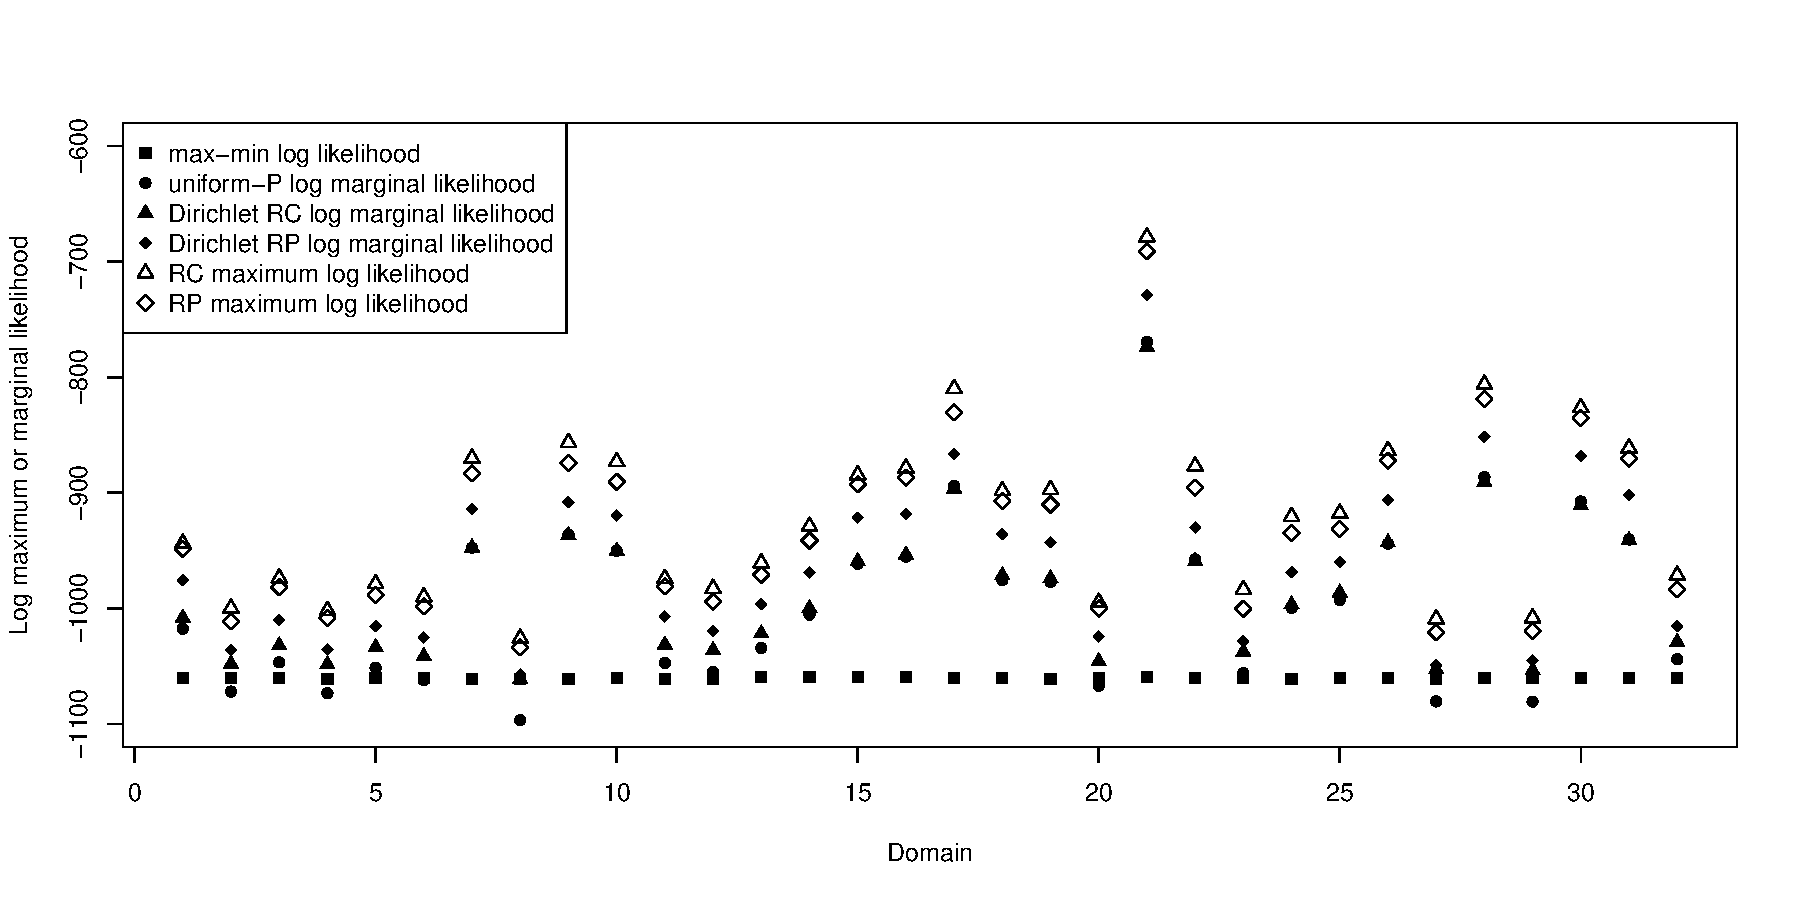
\includegraphics[width=\textwidth]{figures/max_mar_like.pdf}
  \caption{Log maximum and marginal likelihood values for various choice models, by domain.}
  \label{f:max_mar_like}
\end{figure}

\begin{figure}
  \centering
  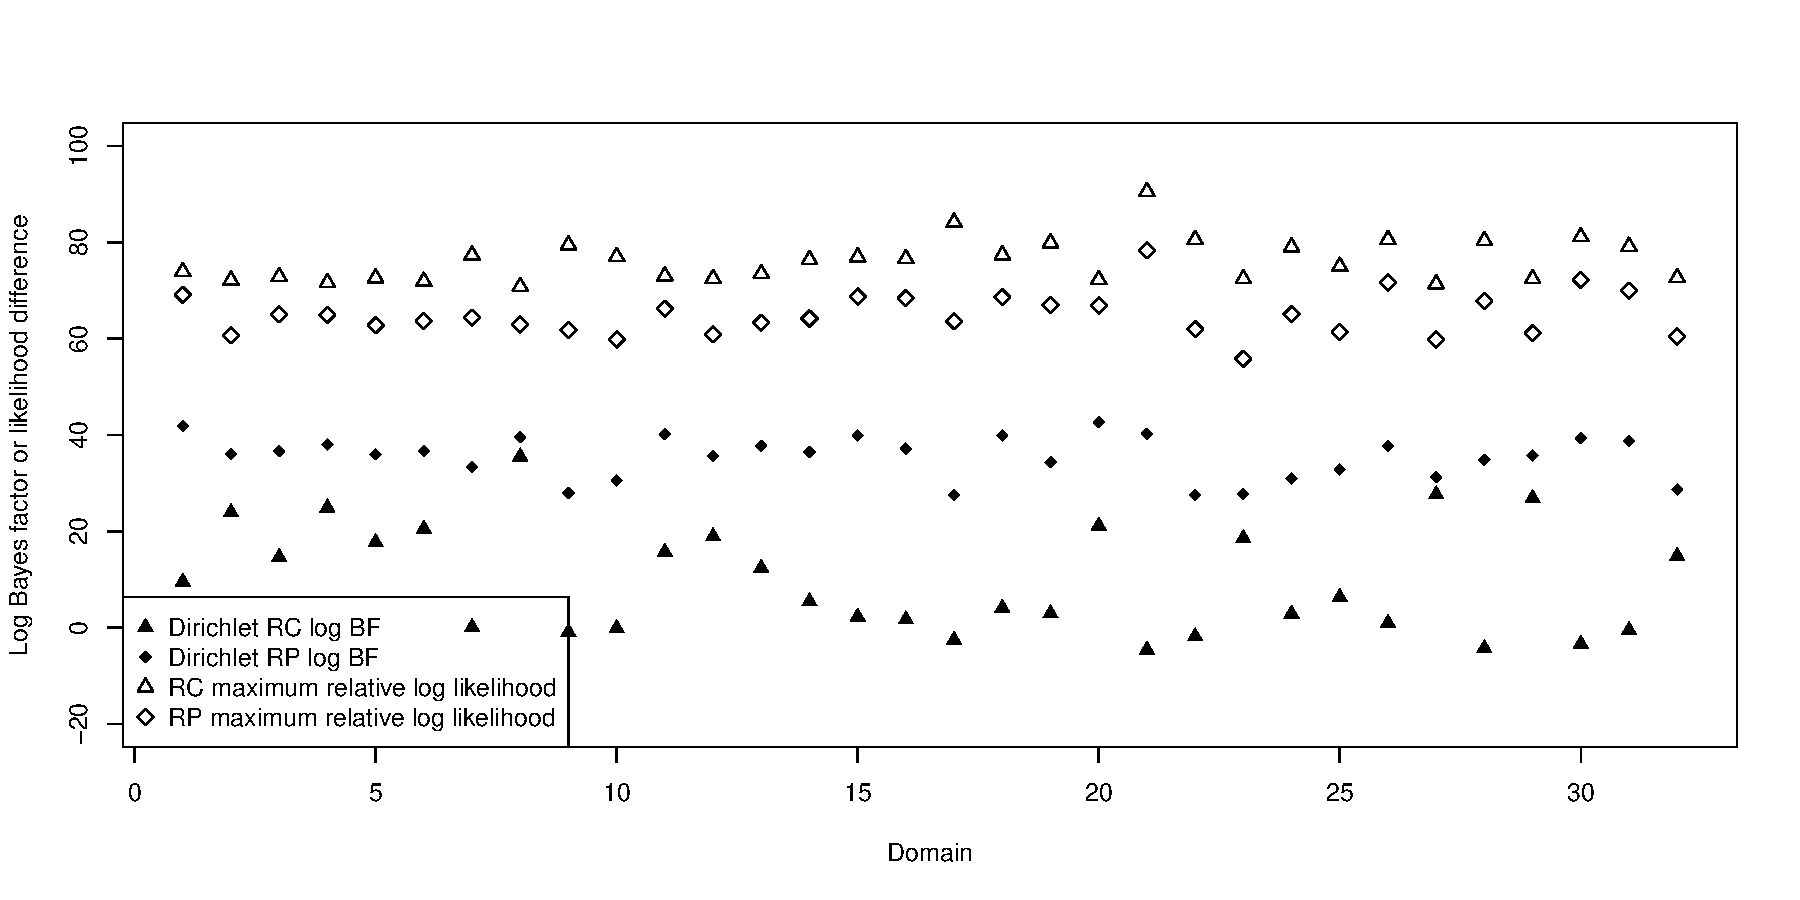
\includegraphics[width=\textwidth]{figures/BF.pdf}
  \caption{Log Bayes factors of the \DP{} and of the \Dpi{}, against the uniform-$P$ model, by domain. Also shown are the difference between the DC maximum log likelihood value and the uniform-$P$ log marginal likelihood and the difference between the DC maximum log likelihood value and the uniform-$P$ log marginal likelihood, by domain.}
  \label{f:BF}
\end{figure}

We now turn to Bayes factors in favour of the hybrid models, against the \DP{}.
We plot the log Bayes factor as a function of $\lambda$ for three domains and tabulate the slope of the log Bayes factor at $\lambda = 1$ for all 32 domains.
The panels on the left of Figure \ref{f:BF_by_lambda} show log Bayes factors in favour of the hybrid model, against the \DP{}, as a function of $\lambda$, for domains 30 (top), 24 (middle), and 23 (bottom).
Standard errors are all less than 0.05.
The supplementary materials include plots for all domains.
The plots for domains 30 and 24 are qualitatively representative of the full set of domains.
For all 32 domains, the Bayes factor is convex for $\lambda$ near 0, becoming concave for larger values of $\lambda$.
For all but one domain, it is monotonically increasing.
The slope at $\lambda = 1$ varies by domain, and is most steep for domain 30 and most shallow for domain 24.
Domain 23 is the only domain for which the Bayes factor is not monotonically increasing, and for this domain, the slope at $\lambda = 1$ is negative.
Even here, however, the Bayes factor is maximized at a value of $\lambda$ fairly close to one, and the maximum value does not greatly exceed the value at $\lambda = 1$.
The panels on the right show the corresponding Bayes factors (not in logs) as a function of $\lambda$.
These can be interpreted as unnormalized posterior densities of $\lambda$ for the hybrid model completed by a prior distribution for $\lambda$ that is uniform on the interval $[0,1]$.

\begin{figure}
  \centering
  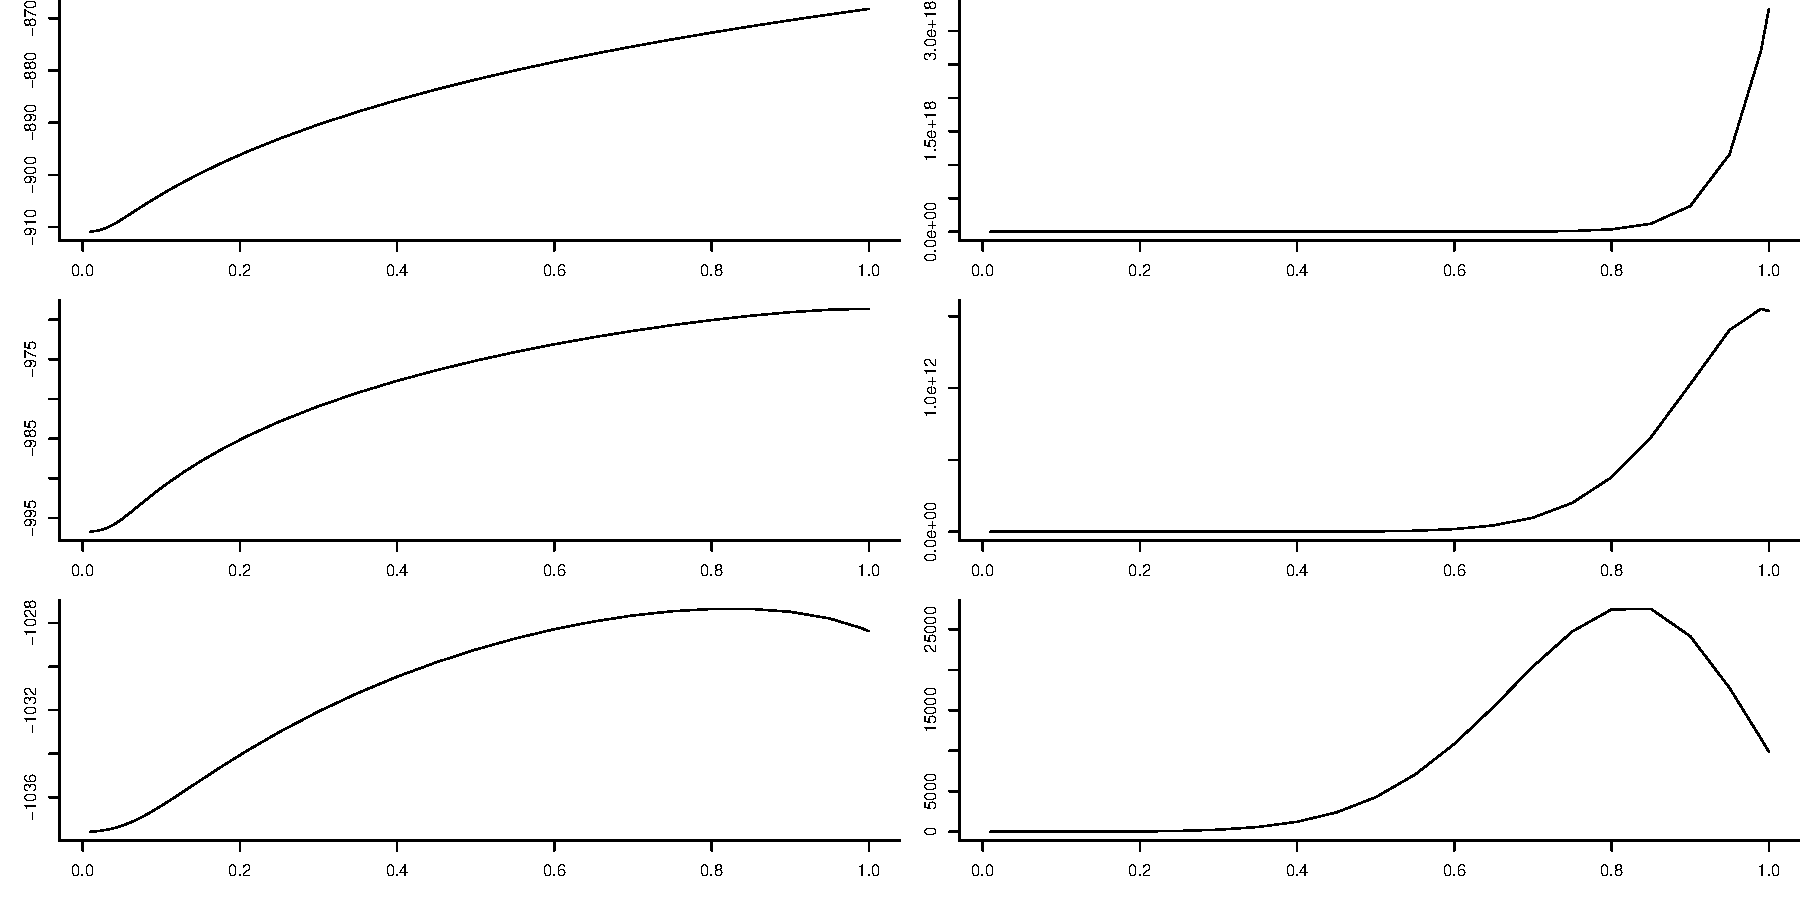
\includegraphics[width=\textwidth]{figures/BF_by_lambda.pdf}
  \caption{Log Bayes factors (left) and Bayes factors (right) by $\lambda$ for domains 30 (top), 24 (middle), and 23 (bottom).}
  \label{f:BF_by_lambda}
\end{figure}

Table \ref{t:BFlike} shows some summary results by domain.
Column 2 gives the maximum number of strictly positive preference probabilities over the set of random preferences maximizing the RP likelihood.
The number varies across domains and is usually, although not always, less than 49, the number of free parameters of a RC model.
Columns 3, 4, and 5 show the numbers of preference probabilities whose posterior mean is greater than $1/n!$, $2/n!$ and $4/n!$.
These gives an idea of the extent to which probability is concentrated on a small number of preferences.
There does not seem to be a strong relationship between these and the maximum number of strictly positive maximum likelihood preferences.
Column 6 gives $\log f_{RC}(y|\hat{P}) - \log \max_\pi f_{RP}(y|\hat{\pi})$, the difference in log maximum likelihood values between the unrestricted RC model and the unrestricted RP model.
Columns 7 and 8 give an estimate of and a numerical standard error for the log Bayes factor $\log[f_{RP}(y)/f_{RC}(y)]$.
These always favour the \Dpi{}, usually very strongly, providing very strong evidence for the \Dpi{} over the alternative \DP{}.
Columns 9 and 10 give an estimate of and a numerical standard error for the derivative of the log Bayes factor $\log[f_\lambda(y)/f_{RC}(y)]$ with repect to $\lambda$, evaluated at $\lambda=1$.
In all but one case, the log Bayes factor in favour of the hybrid model is maximized for $\lambda=1$, which is the \Dpi{}.

\begin{table}
  
\begin{tabular}[t]{rrrrrrrrrr}
\toprule
\multicolumn{1}{c}{ } & \multicolumn{1}{c}{ } & \multicolumn{3}{c}{$E[\pi_i|y]>\ldots$} & \multicolumn{1}{c}{ } & \multicolumn{2}{c}{log Bayes factor} & \multicolumn{2}{c}{log BF slope, $\lambda = 1$} \\
\cmidrule(l{3pt}r{3pt}){3-5} \cmidrule(l{3pt}r{3pt}){7-8} \cmidrule(l{3pt}r{3pt}){9-10}
Domain & $\hat{\pi}_i>0$ & $1/n!$ & $2/n!$ & $4/n!$ & ln like diff & est. & nse & est. & nse\\
\midrule
1 & 34 & 33 & 9 & 6 & 4.83 & 32.38 & 0.014 & 16.99 & 0.038\\
2 & 38 & 40 & 8 & 1 & 11.43 & 12.08 & 0.009 & 4.69 & 0.100\\
3 & 36 & 40 & 12 & 1 & 7.83 & 22.02 & 0.011 & 4.71 & 0.197\\
4 & 34 & 39 & 9 & 2 & 6.65 & 13.11 & 0.011 & 6.46 & 0.103\\
5 & 36 & 36 & 7 & 2 & 9.87 & 18.29 & 0.011 & 9.80 & 0.072\\
\addlinespace
6 & 41 & 36 & 9 & 3 & 8.24 & 16.21 & 0.010 & 9.77 & 0.073\\
7 & 37 & 25 & 14 & 4 & 12.99 & 33.29 & 0.027 & 17.04 & 0.066\\
8 & 33 & 43 & 4 & 0 & 7.87 & 4.01 & 0.008 & 2.65 & 0.063\\
9 & 31 & 25 & 12 & 6 & 17.63 & 28.94 & 0.022 & 15.87 & 0.073\\
10 & 44 & 27 & 11 & 4 & 17.23 & 30.72 & 0.018 & 3.45 & 0.236\\
\addlinespace
11 & 44 & 46 & 8 & 3 & 6.81 & 24.46 & 0.010 & 15.37 & 0.029\\
12 & 49 & 32 & 12 & 2 & 11.62 & 16.73 & 0.011 & 8.57 & 0.061\\
13 & 51 & 39 & 10 & 2 & 10.18 & 25.42 & 0.012 & 15.48 & 0.032\\
14 & 56 & 38 & 13 & 5 & 12.23 & 31.08 & 0.026 & 16.66 & 0.042\\
15 & 53 & 32 & 12 & 4 & 8.23 & 37.67 & 0.033 & 17.39 & 0.054\\
\addlinespace
16 & 31 & 19 & 7 & 3 & 8.19 & 35.52 & 0.020 & 13.75 & 0.118\\
17 & 25 & 16 & 10 & 6 & 20.53 & 30.17 & 0.024 & 4.99 & 0.196\\
18 & 41 & 32 & 12 & 4 & 8.79 & 35.82 & 0.024 & 18.65 & 0.026\\
19 & 32 & 28 & 13 & 3 & 12.87 & 31.45 & 0.027 & 11.46 & 0.111\\
20 & 45 & 50 & 9 & 1 & 5.38 & 21.48 & 0.010 & 13.39 & 0.042\\
\addlinespace
21 & 26 & 28 & 13 & 9 & 12.20 & 44.91 & 0.050 & 20.43 & 0.052\\
22 & 42 & 32 & 16 & 7 & 18.58 & 29.38 & 0.099 & 7.01 & 0.147\\
23 & 37 & 36 & 12 & 2 & 16.58 & 9.21 & 0.015 & -15.00 & 0.284\\
24 & 41 & 26 & 15 & 8 & 13.99 & 28.09 & 0.033 & -0.94 & 0.285\\
25 & 42 & 24 & 4 & 1 & 13.63 & 26.50 & 0.013 & 15.71 & 0.061\\
\addlinespace
26 & 22 & 16 & 7 & 2 & 8.93 & 36.77 & 0.023 & 19.17 & 0.057\\
27 & 33 & 39 & 10 & 2 & 11.54 & 3.59 & 0.014 & 1.96 & 0.128\\
28 & 39 & 26 & 7 & 3 & 12.58 & 39.14 & 0.022 & 18.92 & 0.099\\
29 & 36 & 42 & 10 & 1 & 11.34 & 8.88 & 0.009 & 4.01 & 0.079\\
30 & 38 & 30 & 14 & 4 & 8.96 & 42.70 & 0.023 & 20.76 & 0.048\\
\addlinespace
31 & 45 & 35 & 14 & 7 & 9.21 & 39.36 & 0.028 & 18.69 & 0.056\\
32 & 34 & 25 & 10 & 4 & 12.22 & 13.81 & 0.012 & 3.38 & 0.135\\
\bottomrule
\end{tabular}

  \caption{Summary results by domain. The first column shows the domain index.
The second column shows the maximum number of strictly positive preference probabilities, out of 120, for a random preference that maximizes the RP likelihood.
The third column show the difference between the RC and RP maximum log likelihoods.
The fourth and fifth columns show a numerical estimate of the Bayes factor in favour of the \Dpi{} model over the \DP{} model, and a numerical standard error for this estimate.
The sixth and seventh columns show a numerical estimate of the derivative with respect to $\lambda$ of the Bayes factor in favour of the hybrid model over the \DP{} model, at the value $\lambda = 1$.}
  \label{t:BFlike}
\end{table}

\subsection{Features of posterior distributions.}

Recall that for the \DP{}, the \Dpi{} and all hybrid models, the prior distributions of $\alpha$ are identical.
Also identical are the marginal prior distributions of each $P_A(\cdot)$.
This does not imply that for given $y$, posterior distributions will be identical.
%Table \ref{t:alpha} gives, for each domain and both models, numerical estimates of the posterior mean and standard deviation of $\alpha$, as well as the numerical standard error for the estimate of the mean.
%\begin{table}
%  
\begin{tabular}[t]{rrrrrrr}
\toprule
\multicolumn{1}{c}{ } & \multicolumn{3}{c}{RCM} & \multicolumn{3}{c}{RPM} \\
\cmidrule(l{3pt}r{3pt}){2-4} \cmidrule(l{3pt}r{3pt}){5-7}
Domain & mean & std & nse & mean & std & nse\\
\midrule
1 & 11.75 & 2.83 & 0.026 & 20.46 & 7.54 & 0.110\\
2 & 29.59 & 9.80 & 0.125 & 35.48 & 14.46 & 0.190\\
3 & 17.25 & 4.86 & 0.062 & 21.66 & 8.83 & 0.221\\
4 & 30.80 & 9.95 & 0.133 & 31.48 & 13.62 & 0.265\\
5 & 19.31 & 5.46 & 0.052 & 25.87 & 10.07 & 0.207\\
\addlinespace
6 & 23.90 & 7.28 & 0.113 & 27.67 & 11.48 & 0.247\\
7 & 6.36 & 1.34 & 0.017 & 13.98 & 5.21 & 0.168\\
8 & 57.94 & 19.81 & 0.265 & 48.45 & 20.80 & 0.506\\
9 & 5.54 & 1.19 & 0.012 & 10.82 & 4.25 & 0.095\\
10 & 6.52 & 1.39 & 0.015 & 15.43 & 5.61 & 0.134\\
\addlinespace
11 & 17.39 & 4.79 & 0.058 & 25.87 & 9.79 & 0.143\\
12 & 20.77 & 5.89 & 0.069 & 27.44 & 11.02 & 0.192\\
13 & 14.34 & 3.78 & 0.054 & 22.62 & 8.45 & 0.157\\
14 & 9.20 & 2.21 & 0.022 & 17.91 & 6.39 & 0.174\\
15 & 7.03 & 1.50 & 0.016 & 16.89 & 5.90 & 0.134\\
\addlinespace
16 & 7.00 & 1.52 & 0.017 & 12.61 & 4.78 & 0.121\\
17 & 4.04 & 0.83 & 0.010 & 6.69 & 2.64 & 0.063\\
18 & 7.73 & 1.73 & 0.022 & 17.88 & 6.50 & 0.151\\
19 & 6.78 & 1.56 & 0.014 & 12.15 & 4.72 & 0.087\\
20 & 25.80 & 8.27 & 0.057 & 28.50 & 11.13 & 0.205\\
\addlinespace
21 & 2.52 & 0.49 & 0.005 & 6.19 & 2.36 & 0.057\\
22 & 5.49 & 1.21 & 0.014 & 9.46 & 3.49 & 0.125\\
23 & 20.89 & 6.12 & 0.079 & 25.55 & 10.94 & 0.245\\
24 & 7.69 & 1.90 & 0.019 & 11.20 & 4.17 & 0.092\\
25 & 9.42 & 2.12 & 0.020 & 13.28 & 5.35 & 0.112\\
\addlinespace
26 & 5.70 & 1.24 & 0.010 & 6.92 & 2.61 & 0.047\\
27 & 36.92 & 12.35 & 0.131 & 27.34 & 13.56 & 0.377\\
28 & 4.46 & 0.87 & 0.013 & 9.22 & 3.50 & 0.135\\
29 & 38.51 & 13.29 & 0.137 & 34.46 & 14.53 & 0.274\\
30 & 4.58 & 0.94 & 0.012 & 10.31 & 3.75 & 0.092\\
\addlinespace
31 & 5.77 & 1.23 & 0.015 & 13.78 & 4.87 & 0.085\\
32 & 17.03 & 4.66 & 0.064 & 16.38 & 6.82 & 0.139\\
\bottomrule
\end{tabular}

%  \caption{Posterior mean and standard deviation of $\alpha$, with numerical standard error for the mean, for the \DP{} and the \Dpi{}, by domain}
%  \label{t:alpha}
%\end{table}
Table \ref{t:alpha_q} shows, for each domain and both models, numerical estimates of the posterior quantiles 0.025, 0.5 and 0.975 of $\alpha$ and the numerical standard errors for each quantile.
\begin{table}
  
\begin{tabular}[t]{rrrrrrrrrrrrr}
\toprule
\multicolumn{1}{c}{ } & \multicolumn{6}{c}{RCM} & \multicolumn{6}{c}{RPM} \\
\cmidrule(l{3pt}r{3pt}){2-7} \cmidrule(l{3pt}r{3pt}){8-13}
\multicolumn{1}{c}{ } & \multicolumn{2}{c}{p=0.025} & \multicolumn{2}{c}{p=0.5} & \multicolumn{2}{c}{p=0.975} & \multicolumn{2}{c}{p=0.025} & \multicolumn{2}{c}{p=0.5} & \multicolumn{2}{c}{p=0.975} \\
\cmidrule(l{3pt}r{3pt}){2-3} \cmidrule(l{3pt}r{3pt}){4-5} \cmidrule(l{3pt}r{3pt}){6-7} \cmidrule(l{3pt}r{3pt}){8-9} \cmidrule(l{3pt}r{3pt}){10-11} \cmidrule(l{3pt}r{3pt}){12-13}
Domain & quant & nse & quant & nse & quant & nse & quant & nse & quant & nse & quant & nse\\
\midrule
1 & 7.13 & 0.06 & 11.45 & 0.04 & 18.29 & 0.13 & 8.66 & 0.11 & 19.43 & 0.15 & 38.36 & 0.37\\
2 & 15.69 & 0.13 & 28.18 & 0.14 & 52.63 & 0.50 & 14.19 & 0.24 & 33.18 & 0.35 & 69.72 & 0.72\\
3 & 9.84 & 0.09 & 16.68 & 0.07 & 28.58 & 0.23 & 8.51 & 0.19 & 20.35 & 0.14 & 43.30 & 0.41\\
4 & 16.43 & 0.12 & 29.09 & 0.12 & 55.20 & 0.62 & 11.69 & 0.43 & 28.87 & 0.28 & 63.78 & 0.72\\
5 & 11.26 & 0.07 & 18.66 & 0.05 & 32.10 & 0.32 & 11.11 & 0.23 & 24.79 & 0.16 & 51.25 & 0.54\\
\addlinespace
6 & 13.42 & 0.11 & 22.80 & 0.08 & 40.61 & 0.27 & 11.21 & 0.30 & 26.32 & 0.20 & 54.30 & 0.50\\
7 & 4.13 & 0.02 & 6.24 & 0.02 & 9.40 & 0.06 & 6.07 & 0.10 & 13.22 & 0.09 & 25.33 & 0.28\\
8 & 28.94 & 0.28 & 54.79 & 0.30 & 107.48 & 1.63 & 17.79 & 0.44 & 44.81 & 0.51 & 96.30 & 0.76\\
9 & 3.59 & 0.02 & 5.43 & 0.02 & 8.07 & 0.05 & 4.62 & 0.10 & 10.44 & 0.14 & 20.78 & 0.25\\
10 & 4.24 & 0.02 & 6.42 & 0.02 & 9.70 & 0.06 & 6.77 & 0.11 & 14.59 & 0.15 & 28.28 & 0.29\\
\addlinespace
11 & 9.84 & 0.07 & 16.74 & 0.08 & 28.44 & 0.16 & 10.70 & 0.18 & 24.27 & 0.14 & 47.71 & 0.37\\
12 & 11.71 & 0.06 & 19.92 & 0.09 & 35.21 & 0.35 & 11.13 & 0.21 & 25.74 & 0.20 & 52.98 & 0.56\\
13 & 8.49 & 0.07 & 13.81 & 0.03 & 23.08 & 0.13 & 9.79 & 0.11 & 21.18 & 0.14 & 42.28 & 0.32\\
14 & 5.56 & 0.05 & 8.92 & 0.04 & 14.30 & 0.11 & 7.98 & 0.15 & 17.03 & 0.14 & 32.38 & 0.22\\
15 & 4.45 & 0.03 & 6.88 & 0.02 & 10.43 & 0.07 & 7.70 & 0.12 & 16.06 & 0.14 & 30.22 & 0.24\\
\addlinespace
16 & 4.51 & 0.02 & 6.84 & 0.02 & 10.41 & 0.06 & 5.31 & 0.11 & 12.05 & 0.10 & 23.76 & 0.18\\
17 & 2.68 & 0.02 & 3.95 & 0.01 & 5.90 & 0.03 & 2.63 & 0.09 & 6.36 & 0.06 & 12.81 & 0.13\\
18 & 4.83 & 0.03 & 7.58 & 0.03 & 11.71 & 0.08 & 7.77 & 0.11 & 16.73 & 0.11 & 32.64 & 0.31\\
19 & 4.19 & 0.03 & 6.58 & 0.02 & 10.08 & 0.07 & 5.16 & 0.08 & 11.42 & 0.09 & 23.03 & 0.26\\
20 & 13.81 & 0.10 & 24.41 & 0.11 & 46.66 & 0.52 & 12.08 & 0.18 & 26.92 & 0.17 & 54.45 & 0.51\\
\addlinespace
21 & 1.69 & 0.01 & 2.49 & 0.01 & 3.55 & 0.02 & 2.63 & 0.05 & 5.85 & 0.07 & 11.49 & 0.13\\
22 & 3.48 & 0.02 & 5.38 & 0.02 & 8.22 & 0.05 & 4.06 & 0.09 & 8.77 & 0.10 & 16.91 & 0.19\\
23 & 11.82 & 0.06 & 20.08 & 0.09 & 35.20 & 0.32 & 10.13 & 0.25 & 23.98 & 0.29 & 51.73 & 0.51\\
24 & 4.60 & 0.04 & 7.48 & 0.02 & 12.00 & 0.11 & 4.75 & 0.18 & 10.43 & 0.08 & 20.59 & 0.21\\
25 & 5.86 & 0.04 & 9.11 & 0.03 & 14.13 & 0.09 & 5.30 & 0.12 & 12.56 & 0.10 & 26.09 & 0.28\\
\addlinespace
26 & 3.63 & 0.02 & 5.59 & 0.02 & 8.52 & 0.06 & 2.97 & 0.08 & 6.59 & 0.11 & 13.21 & 0.15\\
27 & 18.81 & 0.15 & 34.89 & 0.18 & 66.19 & 0.83 & 9.81 & 0.30 & 24.96 & 0.36 & 61.60 & 1.26\\
28 & 2.99 & 0.02 & 4.36 & 0.01 & 6.45 & 0.03 & 3.90 & 0.13 & 8.96 & 0.17 & 17.54 & 0.24\\
29 & 19.38 & 0.21 & 36.54 & 0.16 & 71.77 & 0.65 & 13.56 & 0.38 & 31.69 & 0.27 & 68.89 & 0.93\\
30 & 2.99 & 0.02 & 4.50 & 0.01 & 6.67 & 0.04 & 4.56 & 0.07 & 9.89 & 0.09 & 18.89 & 0.18\\
\addlinespace
31 & 3.71 & 0.03 & 5.63 & 0.02 & 8.54 & 0.06 & 5.92 & 0.10 & 13.03 & 0.09 & 24.40 & 0.18\\
32 & 9.83 & 0.07 & 16.43 & 0.06 & 27.93 & 0.25 & 6.52 & 0.18 & 14.88 & 0.23 & 31.89 & 0.38\\
\bottomrule
\end{tabular}

  \caption{Posterior quantiles of $\alpha$, and their numerical standard errors, for the \DP{} and \Dpi{}, by  domain}
  \label{t:alpha_q}
\end{table}
We see that the posterior distribution of $\alpha$ can differ between the \DP{} and the \Dpi{}.
In most, but not all cases, the posterior median of $\alpha$ is greater for the \Dpi{}.
At the same time, the posterior distribution of $\alpha$ is more diffuse, with the posterior quantile 0.025 being smaller and the posterior quantile 0.975 being greater, in most cases.
The supplementary materials include plots of the posterior density of $\alpha$, for both models and each domain.
These show more clearly that in both the right and left tails, the posterior density of $\alpha$ for the \Dpi{} dominates that for the \DP{}.

This attests to the robustness of the empirical support for the \Dpi{}, over the \DP{}, to changes in the prior distribution of $\alpha$.
To defend this claim, we first derive an expression for the conditional Bayes factor $f_{RP}(y|\alpha)/f_{RC}(y|\alpha)$ favouring the \Dpi{} over the \DP{}, for a fixed value of $\alpha$.
Since we use the same prior for $\alpha$ for both models, Bayes rule gives, for any value of $\alpha$, the conditional Bayes factor given $\alpha$ as the product of the unconditional Bayes factor and the ratio of posterior densities of $\alpha$:
\[
  \frac{f_{RP}(y|\alpha)}{f_{RC}(y|\alpha)} = \frac{f_{RP}(y)}{f_{RC}(y)} \cdot \frac{f_{RP}(\alpha|y)}{f_{RC}(\alpha|y)}.
\]
We have already reported results on the unconditional Bayes factor, the first RHS factor, and they favour, usually quite strongly, the \Dpi{}.
For very small or large values of $\alpha$, the second RHS factor is much larger than one, and thus the conditional Bayes factor is much larger than the unconditional Bayes factor.
But the second factor never becomes much less than one.
Because the conditional Bayes factors are never much lower than the unconditional Bayes factor, and are much larger for extreme values of $\alpha$, the results favouring the \Dpi{} over the \DP{} are robust to the choice of prior distribution of $\alpha$.

Figure \ref{f:pi} illustrates some features of the posterior distribution $\pi|y$ for the \Dpi{}, using data from domain 1, ``Male stars''.
Of the $n! = 120$ elements of $\pi$, 10 have a posterior mean greater than $2/n!$.
For these 10 preference probabilities, the left panel shows the posterior mean (circle) and posterior quantiles, for cumulative probabilities 0.25, 0.5, 0.75 and 0.9.
We see that the preference probabilities have highly skewed distributions: the lower quartile is indistinguishable from zero at the resolution of the graphic, and the median is a small fraction of the upper quartile.
All probabilities have a mean below 0.1 and most, a mean below 0.05; their combined mean probability is 0.36.
Collectively, these preferences are fairly important but none are indispensible.
The right panel shows posterior correlations among the ten preference probabilities.
Not surprisingly, similar preferences tend to have negatively correlated probabilities.
We also see patterns arising from non-identification of $\pi$ of the kind illustrated in \possessivecite{Fish99} example.
Take for example, the correlation structure for the preference probabilities $\pi_{acbde}$, $\pi_{cadeb}$, $\pi_{acdeb}$ and $\pi_{cabde}$.
A random preference where $\pi_{acbde} = \pi_{cadeb} = \tfrac{1}{2}$ induces all the same choice probabilities as the random preference where $\pi_{acdeb} = \pi_{cabde} = \tfrac{1}{2}$, as do all mixtures of the two random preferences.
This gives rise to the pattern in the figure where the correlation between $\pi_{acbde}$ and $\pi_{cadeb}$ is positive, the correlation between $\pi_{acdeb}$ and $\pi_{cabde}$ is positive and the four cross-correlations are all negative.
The supplementary materials include two figures like Figure \ref{f:pi} for each domain, one for probabilities whose posterior mean is greater than $2/n!$ (as in Figure \ref{f:pi}) and the other for those whose posterior mean is greater than $1/n!$.

\begin{figure}
  \centering
  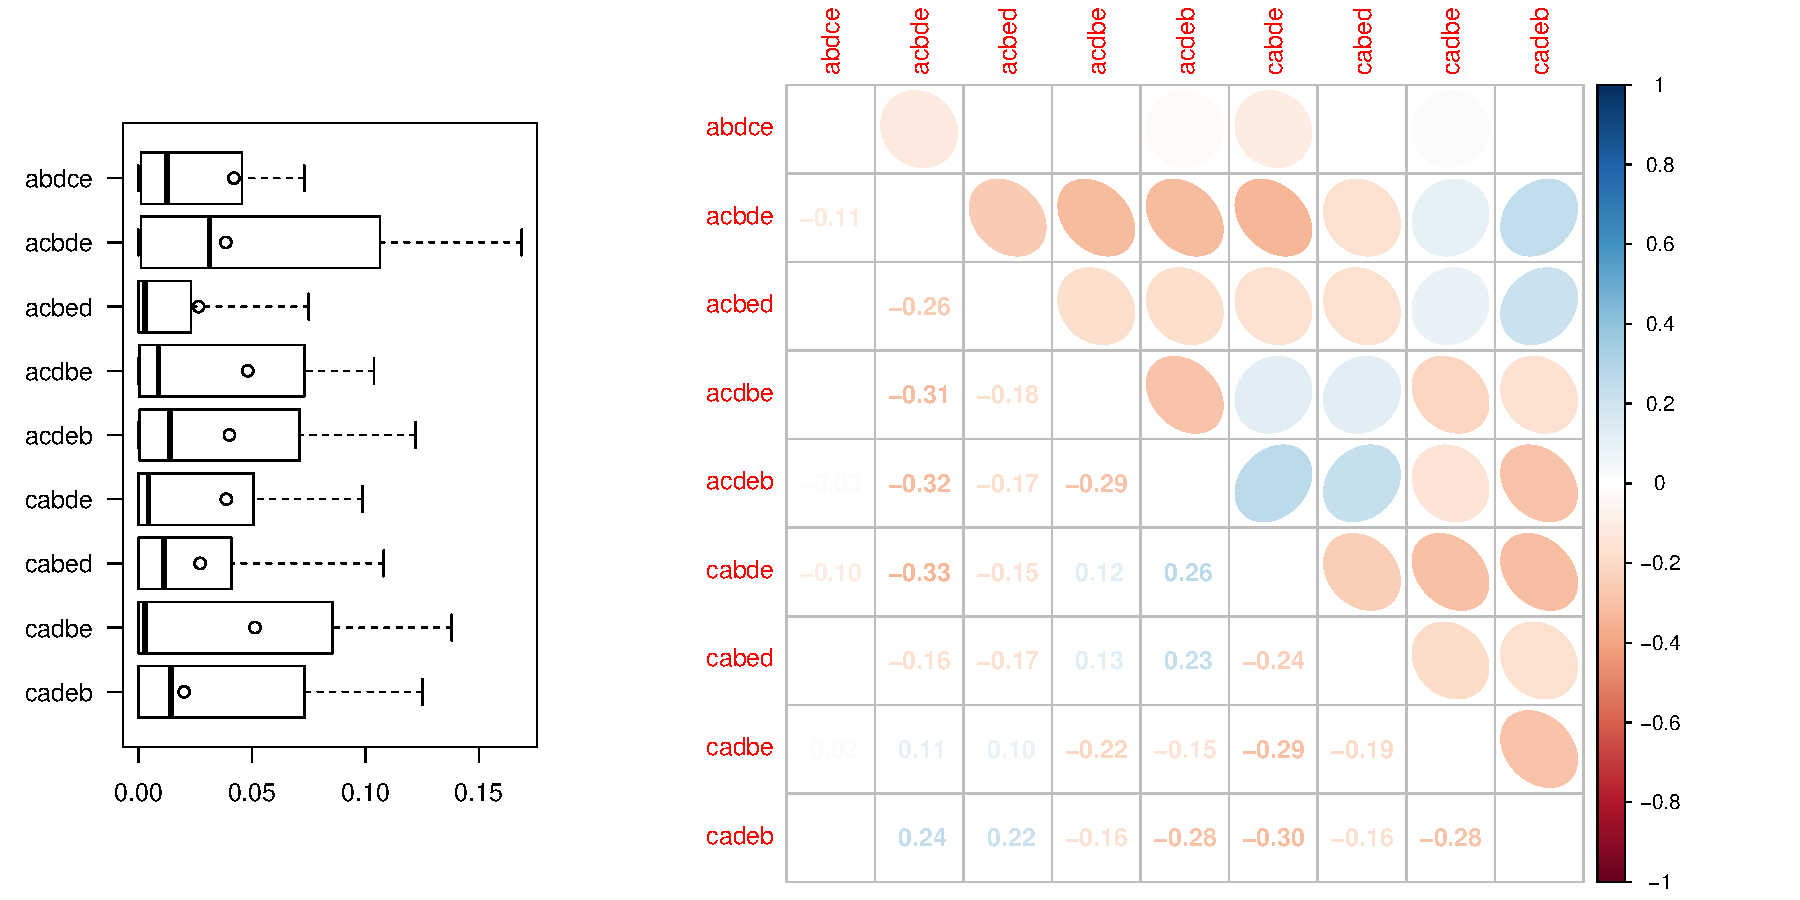
\includegraphics[width=\textwidth]{figures/pi.pdf}
  \caption{Posterior statistics for those preferences probabilities $\pi_\succ$ with posterior mean greater than $2/n!$, using data from domain 1, ``Male stars''.
  Preference indices are strings ranking objects $a$, $b$, $c$, $d$ and $e$ from most to least preferred; thus $abdce$ indexes the preference $\succ$ for which $a \succ b \succ d \succ c \succ e$.
  The left panel shows the posterior mean (circle), and posterior quantiles for cumulative probabilities 0.25 (left side of box), 0.5 (bold vertical bar), 0.75 (right side of box) and 0.9 (whisker).
  The right panel shows posterior correlations of the same preference probabilities.
  Correlations are indicated numerically (lower triangle), by ellipse eccentricity and direction (upper triangle) and by colour (both triangles).}
  \label{f:pi}
\end{figure}

We now show illustrate some features of the posterior distribution of choice probability vectors, for the \DP{} and the \Dpi{}.
This is easiest to do for binary choice probabilities.
Figure \ref{f:bin_plots} shows numerical estimates of posterior densities of binary choice probabilities, for each of the ten doubleton menus of domain 1 (``Male stars'') and both models.
The universe of options is $T = \{a,b,c,d,e\}$, where the indices $a$, $b$, $c$, $d$ and $e$, correspond to Tom Hanks, Kevin Spacey, Morgan Freeman, Leonardo DiCaprio and Christian Bale, respectively.
The figure shows ten panels within a 4 by 4 grid, where rows are associated with the options $a$, $b$, $c$ and $d$ and columns are associated with the options $b$, $c$, $d$ and $e$.
Each panel shows two posterior densities for the probability of choosing the row object when the menu presented consists of the row and column objects.
The density in green (which always has a lower maximum value) gives the density of the binary choice probability for the \DP{} and the density in red gives the same for the \Dpi{}.
For each doubleton menu, the concentration of the posterior distribution for the \Dpi{}, relative to the \Dpi{}, illustrates the degree to which the posterior distribution borrows strength from other menus, by way of the dependence across menus induced by random preferences.
The supplementary materials include similar figures for each domain.

\begin{figure}
  \centering
  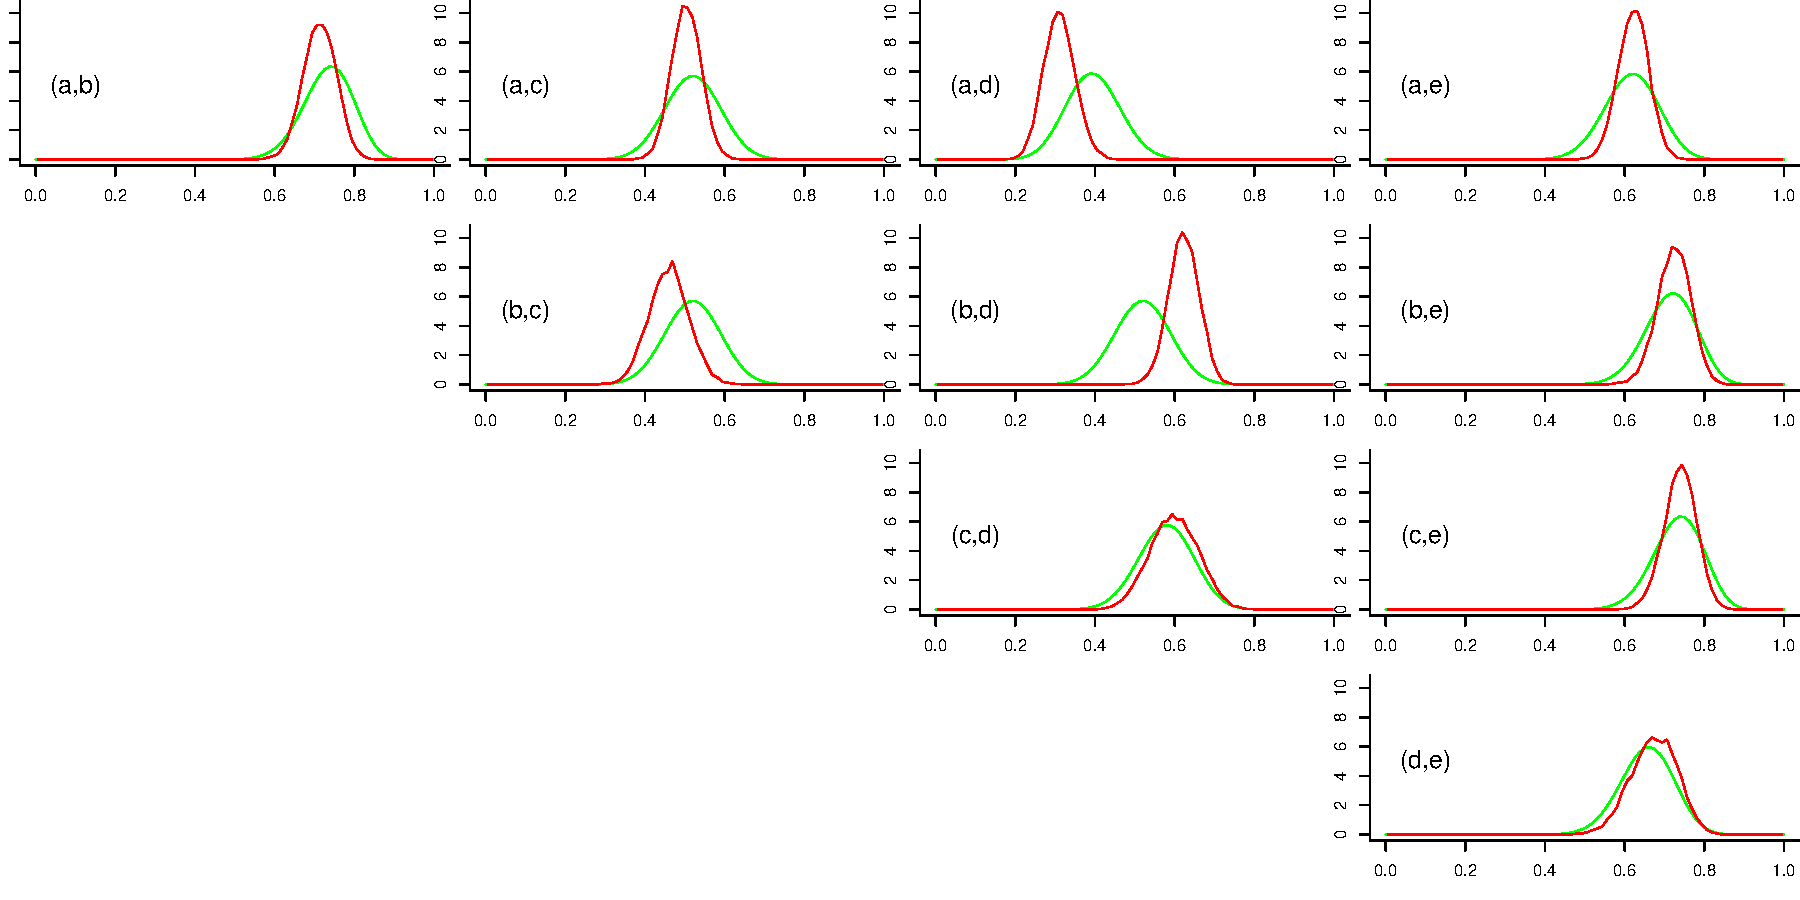
\includegraphics[width=\textwidth]{figures/bin_plots.pdf}
  \caption{Posterior densities of binary choice probabilities for domain 1, for the \DP{} (green) and the \Dpi{} (red). The notation $p(a,b)$, for example, is the probability of choosing option $a$ when options $a$ (Tom Hanks) and $b$ (Kevin Spacey) are presented. The densities for the \Dpi{} always have a higher maximum value. The horizontal and vertical scales are the same for all panels and both models.}
  \label{f:bin_plots}
\end{figure}

Computations were performed on a 2020 Mac mini with the Apple M1 chip.
The supplementary materials provide detailed timing information by domain.
Maximum likelihood computations for a domain took less than $0.8s$, posterior simulation of the \DP{} took less than $0.3s$ and posterior simualtion of the \Dpi{} and hybrid models took between $306s$ and $324s$.

\section{Conclusions}

We have shown that the \Dpi{}, and only it, satisfies three properties that are suitable for inference in an abstract choice setting where we want to treat choice options as {\em a priori} indistinguishable: full support, symmetry in preferences and neutrality with respect to all partitions.
One could make the case for relaxing symmetry in preferences, neutrality with respect to all partitions, or both, in a way that preserves symmetry with respect to choice options, appealing to the fact that the set of permutations has structure even if the set of options does not.
However, there are many ways to add structure to preference distributions, drawing on the structure of permutations, and little theoretical guidance for how to do this.
Here we have decided to follow a simple approach, treating preferences completely symmetrically, leaving the investigation of more structured preference distributions for future research.

For values of $\alpha$ that are reasonable given our empirical results, the symmetric Dirichlet prior density $f_{SD}(\pi|\alpha)$ of the \Dpi{} resembles the spike-and-slab sparseness priors that rein in overfitting in highly flexible models.
The prior shrinks most preference probabilities towards zero and thus favours preference distributions where only a small number of preferences have non-negligible probability.

We have shown how to compute approximations of marginal likelihoods, which measure out-of-sample predictive performance, for the \DP{}, the \Dpi{} and a continuum of hybrid models bridging these two models.
This allows one to use Bayes factors to compare the \Dpi{} against the \DP{} and against the various hybrid models.
In each case, the comparison is particularly clean: all of these models agree on the marginal prior distribution of choice probability vectors $P_A(\cdot)$ and differ only in terms of the dependence structure, which, in the case of the \Dpi{}, is induced by random preferences, and in the case of the \DP{}, is absent.
Comparing the \Dpi{} with the hybrid models allows us to detect certain kinds of evidence against the \Dpi{}, further exposing it to possible falsification.
More broadly, obtaining the marginal likelihood for the \Dpi{} allows us to compare it with {\em any} model for the same data for which one can compute a marginal likelihood.

We applied our methods to experimental data featuring 32 choice domains, and found the evidence in favour of random preference to be quite strong.
In all 32 cases, the \Dpi{} is favoured over the \DP{}, due to its superior out-of-sample predictive performance, measured by log marginal likelihood.
In most cases, the evidence is quite strong.
Furthermore, in 31 out of 32 cases, the \Dpi{} has a higher marginal likelihood than all of the hybrid models and even in the remaining case, the RPM is competitive with the best hybrid model.

The log marginal likelihood of the \Dpi{} bridges, on average, most of the gap between the log marginal likelihood of the \DP{} and the expected log likelihood of the ideal RC model $P_0$.
To help interpret this observation, it is instructive to isolate the features of the \DP{} that account for its poor predictive performance relative to the ideal RC model, and see which of these features also apply, or do not apply, to the \Dpi{} model.
Recall that the \DP{} is based on independent Dirichlet priors for the choice probability vectors $P_A(\cdot)$, menu by menu.
As an abstract choice model local to a single menu, it is hard to beat the Dirichlet-multinomial model, a workhorse Bayesian model for univariate multinomial observations when no conditioning information is available.
Recognizing this allows us to see clearly two distinct features holding back the predictive performance of the \DP{}.
First, as an abstract choice model, it does not exploit information about the attributes of the various choice objects.
Second, given $\alpha$, choice probabilities across menus are {\em a priori} conditionally independent, which precludes any learning across menus in a \DP{} with fixed $\alpha$ and severely limits such learning in a hierarchical model completed by a prior for $\alpha$.
The \Dpi{}, also an abstract choice model, retains the first feature.
However, by building in mutual prior dependence among choice probability vectors $P_A(\cdot)$ (keeping their marginal prior distributions constant) it allows learning across menus.
The fact that it does so in a way that improves predictive performance more than half way towards the expected predictive performance of the ideal RC model, despite being an abstract choice model, is much in its favour.

We contend that now that computing marginal likelihoods for the \Dpi{} is feasible, it serves as a useful minimal standard against which we can compare any RC model, including models that conditional on object attributes, using the choice datasets analysed here or similar choice datasets.
Random preference is intuitively appealing, conceptually simple and well established.
The \Dpi{} has a number of attractive theoretical properties and bridges much of the gap in predictive performance between the \DP{} and the ideal RC model.
We are aware of no other model for which marginal likelihoods are available, and greater, over a wide variety of choice domains.

It will be helpful to consider different kinds of models that might bridge some of the remaining gap between the \Dpi{} and the ideal RC model, while retaining symmetry in objects.
One kind of model retains the full support condition of the \Dpi{} but relaxes symmetry in preferences and/or neutrality with respect to all partitions.
An example is a Mallows model with a latent reference preference whose distribution is symmetric in objects.
Some mixtures of Mallows models would also qualify.
Another kind of model is obtained by truncating the support of the \Dpi{} (or any other Bayesian RP model).
Examples would be models imposing discrete choice axioms on induced choice probabilities, axioms such as weak stochastic transitivity or \possessivecite{sattath:76} multiplicative inequality.
Another example is \possessivecite{ApesBallLu17} single-crossing random utility model (SCRUM).
Yet another kind of model expands rather than restricts possible choice probabilities.
Consider a Bayesian RC model where the support of $P$ goes beyond the random preference region to accommodate, say, asymmetric dominance effects, while maintaining some kind of dependence across the $P_A(\cdot)$ resembling the dependence induced by random preference.
For example, one could truncate the prior for $P$ in a full-support Bayesian RC model to the region where some relaxed version of the Block-Marschak conditions holds.

Although our main objective is computing marginal likelihoods, our simulation methods also provide posterior samples of the unknown parameters, namely the concentration parameter $\alpha$ and the vector $\pi$ of preference probabilities, for the \DP{}, the \Dpi{} and the hybrid models.
From these posterior samples, we can generate posterior samples of various functions of interest, such as the choice probability vectors $P_A(\cdot)$.

Reporting and making sense of the distribution of $\pi$ is a challenge.
The vector $\pi$ is not identified and there are no obvious restrictions that would allow for identification.
Similar preferences induce similar choices.
The number of preferences, $n!$, rises quickly in the number $n$ of choice options.
For the data we have seen, the distributions of individual preference probabilities are highly skewed and probability is spread over a fairly large number of preferences.

\appendix

\section{A Metropolis-Hastings update of blocks of weights}\label{s:gammadraw}

We describe here a Metropolis-Hastings update of the block $\gamma_{[x\cdots]}$, preserving the posterior distribution with density $f_\lambda(\alpha,\gamma|y)$.
The block index $x \in T$ and the hybrid model index $\lambda \in [0,1]$ are arbitrary.
We are conditioning throughout on $\alpha$ and the preference weights outside the block $\gamma_{[x\cdots]}$, which we denote by $\gamma_{-[x\cdots]}$

The update consists of the draw of a proposal $\gamma_{[x\cdots]}^*$, from a time-reversible Markov transition distribution $\gamma_{[x\cdots]}^*|\gamma_{[x\cdots]}$ that preserves the prior distribution of $\gamma_{|x\cdots]}$, followed by a Metropolis-Hastings accept-reject step.
The proposal distribution, defined up to a correlation parameter $\phi \in [0,1]$, is defined by the following procedure, in which the draws of $\beta$, $\epsilon$ and $\pi^*$ are mutually independent, and independent of the current state $\gamma_{[x\cdots]}$:
\begin{enumerate}
    \item Draw $\beta \sim \mathrm{Be}(\phi \alpha/n, (1-\phi) \alpha/n)$ and $\epsilon \sim \mathrm{Ga}((1-\phi) \alpha/n)$.
    \item Compute block sum $\bar\gamma_{[x\cdots]}^* = \beta \bar\gamma_{[x\cdots]} + \epsilon$ for the proposal $\gamma_{[x\cdots]}^*$.
    If the current block sum has distribution $\bar\gamma_{[x\cdots]} \sim \mathrm{Ga}(\alpha/n)$, then the proposed block sum has distribution $\bar\gamma_{[x\cdots]} \sim \mathrm{Ga}(\alpha/n)$. That is, steps 1 and 2 preserve the prior distribution of the block sum $\bar\gamma_{[x\cdots]}$.
    \item Draw $\pi^* \sim \mathrm{Dir}(\alpha/n!,\ldots,\alpha/n!)$, a vector of length $(n-1)!$.
    \item Compute $\gamma_{[x\cdots]}^* = \bar\gamma_{[x\cdots]}^* \pi^*$.
    Note that if $\bar\gamma_{[x\cdots]} \sim \mathrm{Ga}(\alpha/n)$, then the elements of $\gamma_{[x\cdots]}^*$ are independent
    $\mathrm{Ga}(\alpha/n!)$.
\end{enumerate}
Steps 1 and 2 define a distribution $\bar\gamma_{[x\cdots]}^* | \bar\gamma_{[x\cdots]}$ that is the Markov transition distribution for a first order beta-gamma autoregressive (BGAR) process.
The stationary distribution of this Markov transition is identical to the prior distribution of $\bar\gamma_{[x\cdots]}$, which is $\mathrm{Ga}(\alpha/n)$.
See Lewis et al. (1986) for a description of the BGAR, a derivation of its marginal distribution, and a proof that it is time reversible.
The $k$'th order autocorrelation of the process is $\phi^k$.
Steps 3 and 4 draw the elements of the block $\gamma^*_{[x\cdots]}$ from their conditional prior distribution, given their block sum being equal to $\bar\gamma^*_{[x\cdots]}$.
The full sequence of steps 1-4 is time reversible, and preserves the prior distribution of $\gamma_{[x\cdots]}$,
according to which its $(n-1)!$ elements are iid $\mathrm{Ga}(\alpha/n!)$.
Denote by $g(\gamma_{[x\cdots]}^*|\gamma_{[x\cdots]})$ the density of this transition, which we will not need to derive because the transition is time reversible.

After we draw $\gamma_{[x\cdots]}^*$ as described in steps 1-5 above, we accept the proposal with probability $\min(1, H(\gamma_{[x\cdots]}^*,\gamma_{[x\cdots]}))$, where the Hastings ratio is
\[
  H(\gamma_{[x\cdots]}^*,\gamma_{[x\cdots]})
  =
  \frac{g(\gamma_{[x\cdots]}|\gamma_{[x\cdots]}^*)}{g(\gamma_{[x\cdots]}^*|\gamma_{[x\cdots]})}
  \cdot
  \frac{f(\gamma_{[x\cdots]}^*|\alpha) f_\lambda(y|\alpha,\gamma_{[x\cdots]}^*,\gamma_{-[x\cdots]})}
  {f(\gamma_{[x\cdots]}|\alpha) f_\lambda(y|\alpha,\gamma)}
  =
  \frac{f_\lambda(y|\alpha,\gamma_{[x\cdots]}^*,\gamma_{-[x\cdots]})}
  {f_\lambda(y|\alpha,\gamma)}.
\]
The first equation gives the Hastings ratio for the given target density and proposal density.
The second equation provides a important simplification of the Hastings ratio; it follows from the fact that the BGAR is time reversible and its stationary distribution is the prior distribution of $\gamma_{[x\cdots]}$.

\section{Metropolis-Hastings update of $\alpha|\pi,y$}\label{s:alphadraw}

We describe here a Metropolis-Hastings update of the conditional posterior distribution of $\alpha$ given $\pi$ and $y$ (with $G$ marginalized out), for an arbitray fixed value $\lambda \in [0,1]$.
Using the expression for $f(\alpha)$ in \eqref{e:prioralpha} and the expression for $f_{SD}(\pi|\alpha)$ in \eqref{e:priorpi}, we can write the unnormalised target density as
\begin{align*}
  f_\lambda(\alpha|\pi,y)
  \propto f(\alpha) \cdot f_{SD}(\pi|\alpha) \cdot f_\lambda(y|\alpha,\pi)
  &\propto
  \alpha^{a-1} e^{-b\alpha} \cdot
  \frac{\Gamma(\alpha)}{[\Gamma(\tfrac{\alpha}{n!})]^{n!}}
  \left( \prod_{i=1}^{n!} \pi_i^{\tfrac{\alpha}{n!} - 1} \right)
  \cdot f_\lambda(y|\alpha,\pi) \\
  &=
  \alpha^{a-1} \cdot \exp[-(b - \bar{p})\alpha]
  \cdot \frac{\Gamma(\alpha)}{[\Gamma(\tfrac{\alpha}{n!})]^{n!}}
  \cdot f_\lambda(y|\alpha,\pi),
\end{align*}
where
\(
  \bar{p} \equiv \tfrac{1}{n!} \sum_{i=1}^{n!} \log \pi_i.
\)

We draw the proposal $\alpha^* \sim \mathrm{Ga}(\bar{a},\bar{b})$, with $\bar{a}$ and $\bar{b}$ chosen to approximates the conditional distribution $\alpha|\pi$.
We choose to approximate $\alpha|\pi$ rather than $\alpha|\pi,y$ because the factor $f_\lambda(y|\alpha,\pi)$ is difficult to approximate.
However, because we are conditioning on $\pi$, its variation is quite moderate, particularly for $\lambda$ close to 1.

We now use the identity $\Gamma(z+1) = z\Gamma(z)$ to write the target density as proportional to the product of a Gamma density and a relatively slowly varying function:
\[
  f_\lambda(\alpha|\pi,y) \propto
  \alpha^{a+n!-2} \cdot \exp[-(b - \bar{p})\alpha]
  \cdot \frac{\Gamma(\alpha + 1)}{[\Gamma(\tfrac{\alpha}{n!} + 1)]^{n!}}
  \cdot f_\lambda(y|\alpha,\pi).
\]
The log target density is
\begin{equation}\label{e:alphatarget}
  \log f_\lambda(\alpha|\pi,y) = (a+n!-2) \log \alpha - (b - \bar{p}) \alpha
  + \log \Gamma(\alpha + 1) - n! \log \Gamma(\tfrac{\alpha}{n!} + 1)
  + \log f_\lambda(y|\alpha,\pi) + k,
\end{equation}
where $k$ is a constant not depending on $\alpha$, and its derivative with respect to $\alpha$ is
\begin{equation}\label{e:truegrad}
  \frac{\partial \log f_\lambda(\alpha|\pi,y)}{\partial \alpha} =
  \frac{a + n! - 2}{\alpha} - (b-\bar{p})
  + \psi(\alpha + 1) - \psi(\tfrac{\alpha}{n!}+1)
  + \frac{\partial \log f_\lambda(y|\alpha,\pi)}{\partial \alpha},
\end{equation}
where $\psi(\cdot)$ is the digamma function, the derivative of the log gamma function $\log \Gamma(\cdot)$.
For $z \geq 0$, $\psi(z+1)$ is well behaved for our purposes.
It is strictly increasing and concave.
For $z \in [0,100]$, its values increase from minus Euler's constant (about -0.577) to about 4.600, and its derivative decreases from about 1.645 to about 0.010.

At each draw, we need to find $\bar{a}$ and $\bar{b}$, as functions of $\pi$, so that the proposal density approximates the density $f(\alpha|\pi)$.
The first step is to find the mode $\bar\alpha$ of $\alpha|\pi$, which is the unique root of the function $h(\alpha) = (a + n! -2)/\alpha -(b-\bar p) + \psi(\alpha + 1) - \psi(\tfrac{\alpha}{n!} + 1)$.
To show that $h(\alpha)$ has a unique root, we note that $h(\alpha)$ is continuous and decreasing,
$\lim_{\alpha \to 0} h(\alpha) = \infty$, and
$\lim_{\alpha \to \infty} h(\alpha) = -(b-\bar p) + \log n!$.
Because $\bar p$ is maximized for $\pi = (1/n!,\ldots,1/n!)$,
$\bar p \leq -\log n!$ and so $\lim_{\alpha \to \infty} h(\alpha) \leq -b < 0$.

The next step is to compute $\psi(\bar\alpha + 1) - \psi(\tfrac{\bar\alpha}{n!} + 1)$.
Fortunately, the conditional distribution $\alpha|\pi$, and therefore its mode $\bar\alpha$, depends on $\pi$ only through the scalar value $\bar p$.
We use a table lookup to find a close approximation of $\bar\alpha$, having precomputed (before any simulation)
$\psi(\bar\alpha + 1) - \psi(\tfrac{\bar\alpha}{n!} + 1)$ on a grid of values of $\bar p$, for given fixed values of the prior hyperparameters $a$ and $b$.

Next, we compute the parameters $\bar a$ and $\bar b$ of the proposal distribution $\mathrm{Ga}(\bar{a},\bar{b})$ as
\[
  \bar{a} = a + \delta_a + n! - 2 \quad \mbox{and} \quad
  \bar{b} = b - \bar{p}
  - \psi(\bar\alpha + 1) + \psi(\tfrac{\bar\alpha}{n!} + 1) + \tfrac{\delta_a}{\bar\alpha},
\]
where $\delta_a = -2$.
The term $\delta_a$ in the expression for $\bar a$ is introduced to capture variation of the term $\log \Gamma(\alpha + 1) - n! \log \Gamma(\tfrac{\alpha}{n!} + 1)$ as a function of $\log \alpha$.
The term $\delta/\bar\alpha$ in the expression for $\bar b$ is introduced so that the mode of the proposal matches the mode of $\alpha|\pi$.
We denote the proposal density $g(\alpha;\bar a, \bar b)$.

After drawing the proposal $\alpha^* \sim \mathrm{Ga}(\bar a, \bar b)$, we accept it with probability $\min(1, H(\alpha^*, \alpha))$, where the Hastings ratio $H(\cdot,\cdot)$ is given by
\[
  H(\alpha^*,\alpha) = \frac{f_\lambda(\alpha^*|\pi,y)}{f_\lambda(\alpha|\pi,y)}
  \cdot \frac{g(\alpha;\bar a,\bar b)}{g(\alpha^*;\bar a, \bar b)}
  = \frac{f(\alpha^*) f(\pi|\alpha^*) f_\lambda(y|\alpha^*,\pi)}
  {f(\alpha) f(\pi|\alpha) f_\lambda(y|\alpha,\pi)}
  \cdot \frac{g(\alpha;\bar a, \bar b)}{g(\alpha^*;\bar a, \bar b)}.
\]
Using the log proposal density, given by
\[
  \log g(\alpha;\bar a, \bar b)
  = (\bar a - 1) \log \alpha - \bar b \alpha
  = (a + \delta_a + n! - 2) \log \alpha
  - [b-\bar{p} - \psi(\bar\alpha + 1) + \psi(\tfrac{\bar\alpha}{n!} + 1)
  + \tfrac{\delta_a}{\bar\alpha}] \alpha,
\]
we can simplify to obtain
\[
  \log \frac{f(\alpha) f(\pi|\alpha)}{g(\alpha;\bar a, \bar b)}
  = \log \Gamma(\alpha + 1) - n! \log \Gamma(\tfrac{\alpha}{n!} + 1)
  - \delta_a \log \alpha - [\psi(\bar\alpha + 1) - \psi(\tfrac{\bar\alpha}{n!} - 1)
  - \tfrac{\delta_a}{\bar\alpha}] \alpha + k,
\]
\begin{equation}\begin{aligned}
  \log H(\alpha^*,\alpha)
  &= \log \Gamma(\alpha^* + 1) - n! \log \Gamma(\tfrac{\alpha^*}{n!} + 1)
  - \log \Gamma(\alpha + 1) + n! \log \Gamma(\tfrac{\alpha}{n!} + 1) \\
  &+ \log f_\lambda(y|\alpha^*,\pi) - \log f_\lambda(y|\alpha,\pi) \\
  &- \delta_a (\log \alpha^* - \log \alpha)
  - [\psi(\bar\alpha + 1) - \psi(\tfrac{\bar\alpha}{n!} + 1)
  - \tfrac{\delta_a}{\bar\alpha}] (\alpha^* - \alpha).
\end{aligned}\end{equation}

\bibliographystyle{oupecon}
\bibliography{bibliography}

\end{document}

\section{Out-takes}

Now condition on $\alpha$; since $\pi \sim \mathrm{Dir}(\alpha/n!,\ldots,\alpha/n!)$ and $G \sim \mathrm{Ga}(\alpha)$ are independent, the weights $\gamma_i$ are iid $\mathrm{Ga}(\alpha/n!)$.
We exploit this fact in our MCMC design at the M phase, where we update $\alpha$, $\pi$ and $G$ from the posterior distribution with density $f_\lambda(\alpha,\pi,G|y)$, for the current value of $\lambda$.
Our MCMC transition consists of two Gibbs blocks.
In the first block, described in detail in Appendix \ref{s:gammadraw}, we update $\gamma$ from the distribution with density $f_\lambda(\gamma|\alpha,y)$.
We use Metropolis-Hastings updates of subvectors of $\gamma$, using proposals from their prior distribution.
Here we exploit the conditional independence of the $\gamma_i$ given $\alpha$.
In the second block, described in detail in Appendix \ref{s:alphadraw}, we update $\alpha$ in way that preserves the distribution with density $f_\lambda(\alpha|\pi,y)$ (n.b. with $G$ marginalized out) and then draw $G \sim \mathrm{Ga}(\alpha)$.
Thus, even though there is posterior dependence between $\alpha$ and $G$, introducing $G$ does not reduce numerical efficiency.

The intuition for defining these blocks comes from the fact that for a given block, there are a large number of menus for which all preferences in the block agree on the most preferred element.
For example, take $n = 5$ and two arbitrary distinct options $x,y \in T$.
Knowing $\succ\, \in R_{[x\cdots]}$ suffices to determine the most preferred option from 4 out of 10 doubleton menus (that it, ${5 \choose 2} - {4 \choose 2}$ out of ${5 \choose 2}$), 6 out of 10 tripletons, 4 out of 5 quads and the only quint.
Knowing that $\succ\, \in R_{[xy\cdots]}$ suffices for 7 out of 10 doubletons, 9 out of 10 tripletons, all 5 quads and the quint.
